% Template for PLoS
% Version 3.1 February 2015
%
% To compile to pdf, run:
% latex plos.template
% bibtex plos.template
% latex plos.template
% latex plos.template
% dvipdf plos.template
%
% % % % % % % % % % % % % % % % % % % % % %
%
% -- IMPORTANT NOTE
%
% This template contains comments intended 
% to minimize problems and delays during our production 
% process. Please follow the template instructions
% whenever possible.
%
% % % % % % % % % % % % % % % % % % % % % % % 
%
% Once your paper is accepted for publication, 
% PLEASE REMOVE ALL TRACKED CHANGES in this file and leave only
% the final text of your manuscript.
%
% There are no restrictions on package use within the LaTeX files except that 
% no packages listed in the template may be deleted.
%
% Please do not include colors or graphics in the text.
%
% Please do not create a heading level below \subsection. For 3rd level headings, use \paragraph{}.
%
% % % % % % % % % % % % % % % % % % % % % % %
%
% -- FIGURES AND TABLES
%
% Please include tables/figure captions directly after the paragraph where they are first cited in the text.
%
% DO NOT INCLUDE GRAPHICS IN YOUR MANUSCRIPT
% - Figures should be uploaded separately from your manuscript file. 
% - Figures generated using LaTeX should be extracted and removed from the PDF before submission. 
% - Figures containing multiple panels/subfigures must be combined into one image file before submission.
% For figure citations, please use "Fig." instead of "Figure".
% See http://www.plosone.org/static/figureGuidelines for PLOS figure guidelines.
%
% Tables should be cell-based and may not contain:
% - tabs/spacing/line breaks within cells to alter layout or alignment
% - vertically-merged cells (no tabular environments within tabular environments, do not use \multirow)
% - colors, shading, or graphic objects
% See http://www.plosone.org/static/figureGuidelines#tables for table guidelines.
%
% For tables that exceed the width of the text column, use the adjustwidth environment as illustrated in the example table in text below.
%
% % % % % % % % % % % % % % % % % % % % % % % %
%
% -- EQUATIONS, MATH SYMBOLS, SUBSCRIPTS, AND SUPERSCRIPTS
%
% IMPORTANT
% Below are a few tips to help format your equations and other special characters according to our specifications. For more tips to help reduce the possibility of formatting errors during conversion, please see our LaTeX guidelines at http://www.plosone.org/static/latexGuidelines
%
% Please be sure to include all portions of an equation in the math environment.
%
% Do not include text that is not math in the math environment. For example, CO2 will be CO\textsubscript{2}.
%
% Please add line breaks to long display equations when possible in order to fit size of the column. 
%
% For inline equations, please do not include punctuation (commas, etc) within the math environment unless this is part of the equation.
%
% % % % % % % % % % % % % % % % % % % % % % % % 
%
% Please contact latex@plos.org with any questions.
%
% % % % % % % % % % % % % % % % % % % % % % % %

\documentclass[10pt,letterpaper]{article}
\usepackage[top=0.85in,left=2.75in,footskip=0.75in]{geometry}

% Use adjustwidth environment to exceed column width (see example table in text)
\usepackage{changepage}
\usepackage{float}

% Use Unicode characters when possible
\usepackage[utf8]{inputenc}
%\usepackage[T1]{fontenc}  % if needed
\usepackage{graphicx}
\usepackage{url}
\usepackage{hyperref}
\usepackage{enumitem}
\usepackage{booktabs}
\usepackage{makecell}


% textcomp package and marvosym package for additional characters
\usepackage{textcomp,marvosym}

% fixltx2e package for \textsubscript
\usepackage{fixltx2e}

% amsmath and amssymb packages, useful for mathematical formulas and symbols
\usepackage{amsmath,amssymb}

% cite package, to clean up citations in the main text. Do not remove.
\usepackage{cite}

% Use nameref to cite supporting information files (see Supporting Information section for more info)
\usepackage{nameref,hyperref}

% line numbers
\usepackage[right]{lineno}

% ligatures disabled
\usepackage{microtype}
\DisableLigatures[f]{encoding = *, family = * }

% rotating package for sideways tables
\usepackage{rotating}

% Remove comment for double spacing
%\usepackage{setspace} 
%\doublespacing

% Text layout
\raggedright
\setlength{\parindent}{0.5cm}
\textwidth 5.25in 
\textheight 8.75in

% Bold the 'Figure #' in the caption and separate it from the title/caption with a period
% Captions will be left justified
\usepackage[aboveskip=1pt,labelfont=bf,labelsep=period,justification=raggedright,singlelinecheck=off]{caption}


\usepackage[table]{xcolor}


% Use the PLoS provided BiBTeX style
\bibliographystyle{plos2015}

% Remove brackets from numbering in List of References
\makeatletter
\renewcommand{\@biblabel}[1]{\quad#1.}
\makeatother

% Leave date blank
\date{}

% Header and Footer with logo
\usepackage{lastpage,fancyhdr,graphicx}
\usepackage{epstopdf}
\pagestyle{myheadings}
\pagestyle{fancy}
\fancyhf{}
\lhead{
\includegraphics[width=2.0in]{PLOS-submission.eps}}
\rfoot{\thepage/\pageref{LastPage}}
\renewcommand{\footrule}{\hrule height 2pt \vspace{2mm}}
\fancyheadoffset[L]{2.25in}
\fancyfootoffset[L]{2.25in}
\lfoot{\sf PLOS}

%% Include all macros below

\newcommand{\lorem}{{\bf LOREM}}
\newcommand{\ipsum}{{\bf IPSUM}}



\definecolor{light-gray}{gray}{0.95}
\newcommand{\code}[1]{\colorbox{light-gray}{\texttt{#1}}}
\newcommand{\codewhite}[1]{\colorbox{white}{\texttt{#1}}}

%% END MACROS SECTION


\begin{document}
\vspace*{0.35in}

% Title must be 250 characters or less.
% Please capitalize all terms in the title except conjunctions, prepositions, and articles.
\begin{flushleft}
{\Large
\textbf\newline{Personalized Prognostic Models for Oncology: A Machine Learning Approach}
}
\newline
% Insert author names, affiliations and corresponding author email (do not include titles, positions, or degrees).
\\
David Dooling\textsuperscript{1,\Yinyang},
%Patti  Green\textsuperscript{1,\ddag},
Angela  Kim\textsuperscript{1,\ddag},
Barbara McAneny\textsuperscript{1,\ddag},
%Doug Scroggin\textsuperscript{1,\ddag},
%Laura Stevens\textsuperscript{1,\ddag},
Jennifer Webster\textsuperscript{1,\Yinyang}
\\
\bigskip
\bf{1} Innovative Oncology Business Solutions, Albuquerque, NM, USA
\\
%\bf{2} Innovative Oncology Business Solutions, Albuquerque, NM, USA
%\\
%\bf{3} Affiliation Dept/Program/Center, Institution Name, City, State, Country
%\\
\bigskip

% Insert additional author notes using the symbols described below. Insert symbol callouts after author names as necessary.
% 
% Remove or comment out the author notes below if they aren't used.
%
% Primary Equal Contribution Note
\Yinyang These authors contributed equally to this work.

% Additional Equal Contribution Note
% Also use this double-dagger symbol for special authorship notes, such as senior authorship.
\ddag These authors also contributed equally to this work.

% Current address notes
%\textcurrency a Insert current address of first author with an address update
% \textcurrency b Insert current address of second author with an address update
% \textcurrency c Insert current address of third author with an address update

% Deceased author note
%\dag Deceased

% Group/Consortium Author Note
%\textpilcrow Membership list can be found in the Acknowledgments section.

% Use the asterisk to denote corresponding authorship and provide email address in note below.
* ddooling@innovativeobs.com

\end{flushleft}
% Please keep the abstract below 300 words
\section*{Abstract}
%Lorem ipsum dolor sit amet, consectetur adipiscing elit. Curabitur eget porta erat. Morbi %consectetur est vel gravida pretium. Suspendisse ut dui eu ante cursus gravida non sed sem. %Nullam sapien tellus, commodo id velit id, eleifend volutpat quam. Phasellus mauris velit, %dapibus finibus elementum vel, pulvinar non tellus. Nunc pellentesque pretium diam, quis %maximus dolor faucibus id. Nunc convallis sodales ante, ut ullamcorper est egestas vitae. Nam %sit amet enim ultrices, ultrices elit pulvinar, volutpat risus.
We have applied a little-known data transformation to subsets of the Surveillance, 
Epidemiology, and End Results (SEER) publically available data of the National Cancer 
Institute (NCI) to make it suitable input to standard machine learning classifiers. This transformation properly treats the right-censored data in the SEER data and the resulting Random Forest and Multi-Layer Perceptron models predict full survival curves. Treating the 6, 12, and 60 months points of the resulting survival curves as 3 binary classifiers, the 18 resulting classifiers have AUC values ranging from  .765 to .885. Further evidence that the models have generalized well from the training data is provided by the extremely high levels of agreement between the random forest and neural network models predictions on the 6, 12, and 60 month binary classifiers.



% Please keep the Author Summary between 150 and 200 words
% Use first person. PLOS ONE authors please skip this step. 
% Author Summary not valid for PLOS ONE submissions.   
\section*{Author Summary}
Lorem ipsum dolor sit amet, consectetur adipiscing elit. Curabitur eget porta erat. Morbi consectetur est vel gravida pretium. Suspendisse ut dui eu ante cursus gravida non sed sem. Nullam sapien tellus, commodo id velit id, eleifend volutpat quam. Phasellus mauris velit, dapibus finibus elementum vel, pulvinar non tellus. Nunc pellentesque pretium diam, quis maximus dolor faucibus id. Nunc convallis sodales ante, ut ullamcorper est egestas vitae. Nam sit amet enim ultrices, ultrices elit pulvinar, volutpat risus.

\linenumbers

\section*{Introduction}
\label{sec:introduction}
%Lorem ipsum dolor sit~\cite{bib1} amet, consectetur adipiscing elit. Curabitur eget porta erat. %Morbi consectetur est vel gravida pretium. Suspendisse ut dui eu ante cursus gravida non sed %sem. Nullam Eq.~(\ref{eq:schemeP}) sapien tellus, commodo id velit id, eleifend volutpat %quam. Phasellus mauris velit, dapibus finibus elementum vel, pulvinar non tellus. Nunc %pellentesque pretium diam, quis maximus dolor faucibus id.~\cite{bib2} Nunc convallis sodales %ante, ut ullamcorper est egestas vitae. Nam sit amet enim ultrices, ultrices elit pulvinar, %volutpat risus.


Opportunities are emerging in many indutries today to develop and deploy services that cater to individual needs and preferences. Music afficianados can create their own radio stations from Pandora\footnote{Pandora Internet Radio - Listen to Free Music You'll Love, \url{http://www.pandora.com/} (accessed 27 Jan 2016)}, bibliophiles can receive 
book recommendations from goodreads.com\footnote{Share Book Recommendations With Your Friends, Join Book Clubs, Answer Trivia, \url{https://www.goodreads.com/} (accessed 27 Jan 2016)}, and Google will provide directions between any two points, giving options such as mode of transportation and warnings of delays in realtime.\footnote{Google Maps, \url{https://goo.gl/lD7Jwf} (accessed 27 Jan 2016)}
These individualized services share many common features. In particular, they leverage large databases to learn and extract information relevant to individuals.  
A class of techniques that transforms data into actionable information goes by the name of Machine Learning \cite{pythonmachinelearning}.
Machine Learning has recently become a popular method to answer questions and solve problems that are too complex to solve via traditional methods. 



The primary objective of this study is to show how machine learning methods can be trained to produce personalized survival prognosis curves. The methods presented below can be applied to any type of survival data. Traditionally, cancer survival curves have been estimated using Kaplan-Meier methods~\cite{cam}. Kaplan-Meier methodology also uses large datasets to make predictions, but the resulting curves are summaries for a population and not necessarily relevant or particularly accurate for any given individual. This propery of Kaplan-Meier methods is exacerbated when dealing with heterogeneous populations.  The methods presented in this report generate personalized survival curves relevant to individual patients. This objective is aligned with Predictive, Preventive and Personalized Medicine (PPPM), which aims to leverage increasing amounts of health data to maximize quality of care and to eliminate inefficient use of resources~\cite{VanPoucke2016}.
%The situation is analgous to consulting the paper copy of the New York Time's bestseller list for your next book%\footnote{\url{http://www.nytimes.com/best-sellers-books/}} and throwing it in the trash because nothing is appealing, or %taking recommendations from your personalized Amazon "recommended for you'' service.
This capability to provide individualized survival curve prognosis is a direct result of the recent advances in computing power and machine learning algorithms, and similar methodology is becoming commonplace in many industries.
 These techniques are now infiltrating the healthcare industry.
 



The Surveillance, Epidemiolgy, and End Results (SEER) Program of the National Cancer Institute (NCI) has been collecting data since 1973.
Intuitively 
researchers feel confident
 that this data will allow researches to detect information crucial to patients and providers, including the relationships between the collected data (demographics, staging, treatment and disease characteristics) and survival outcomes.
Though these relationships evade capture by traditional methods, it is possible to surface them with two machine learning techniques known as \emph{Random Forests} and \emph{Neural Networks}.

The SEER program is the most recognized authoritative source of information on cancer incidence and survival in the United States. SEER currently collects and publishes cancer incidence and survival data from population-based cancer registries covering approximately 28 percent of the US population.


%Quoting directly from the SEER
%website \cite{seerwebsite}:

%\begin{quote}
%The SEER program registries routinely collect data on patient demographics, primary tumor %site, tumor morphology and stage at diagnosis, first course of treatment, and follow-up for vital %status. This program is the only comprehensive source of population-based information in the %United States that includes stage of cancer at the time of diagnosis and patient survival data. %The mortality data reported by SEER are provided by the National Center for Health Statistics. %The population data used in calculating cancer rates is obtained periodically from the Census %Bureau. Updated annually and provided as a public service in print and electronic formats, %SEER data are used by thousands of researchers, clinicians, public health officials, legislators, %policymakers, community groups, and the public.
%\end{quote}


One challenge of the SEER data that is shared by many survival datasets is the inclusion of censored data.
Observations are labeled censored when the survival information is incomplete.
 The SEER data contains the number of months each patient survived, as well as the vital status.
Traditional methods to deal effectively with this kind of "right-censored data'' include Kaplan-Meier curves
and Cox Proportional Hazard models \cite{cam}. 
%The Kaplan-Meier techniques only give estimates for cohorts of patients and are not applicable %for predicting the surival curve for a single patient, and the Cox Proportional Hazard models %require a fairly restrictive set ot assumptions to be satisifed in order to yield reliable results. 
%The Cox Proportional Hazard models are not able to capture the nonlinear relationships %between the given data fields that %go into making predictions; they can only capture the %first-order linear relationships.

Previous work applying machine learning methods to subsets of the SEER data include creative attempts to deal with the problems presented by right-censored data. Shin et al.~\cite{ISI:000337467400005} use semi-supervised learning techniques to predict 5 year survival, essentially imputing values for SEER records where the survival infomation is censored at a value less than 5 years. Zolbanin et al.~\cite{ISI:000355882700012} remove all records corresponding to patients who were living but censored within the 60 month study window. This treatment biases the predictions and leads to overly pessimistic predictions. 

%investigate the effects of comordbidities; i.e., patients with two different cancer diagnosises, %but their treatment of the censored data underestimates the survival probabilities. All records %representing patients who survived at least 60 months as well as all those who died earlier %than 60 months were considered, but patients alive prior to 60 months but censored out of the %study before 60 months were not included. This treatment biases the data and the predictions, %leading to overly pessimistic survival probablilites predicted by the models.


Previous work applying machine learning methods based on decision trees to survival data in general have a long history, starting with Gordon et al.~\cite{Gordon19851065}. A summary of more recent developments concerning \emph{survival trees} is provided by Bou-Hamad et al.~\cite{Bou-Hamad201144}. These methods focus on altering the splitting critieria used in decision tree growth to account for the censoring, and use 1958 Kaplan-Meier methods at the resulting nodes for prediction purposes. These methods do not generalize to non-tree-based machine learning algorithms, though Ishwaran et al. have extended the methodology to \emph{random survival forests}, ensembles of \emph{survival trees}~\cite{Ishwaran20101056}.



 Instead of modifying existing learning algorithms, we focus attention on the input data. This approach allows us to take advantage of powerful and rapidly improving machine learning derived discrete classifiers without modification. 
 The essential idea is to recast the problem as a discrete classification problem (predicting the liklihood that a patient is alive in any given month) instead of a regression problem (predicting survival months). Treating months after diagnosis as just another discrete feature, the SEER data (or any other right-censored data) can be transformed to make predictions for the hazard function (
 probability of dying in the next month, given that the patient has not yet died).
The survival function can then be derived from the hazard function.
%Details of this transformation can be found in this blog post \cite{kuhn} and are presented in %section~(\ref{subsec:transformation}).


%This paper is organized as follows. We introduce the subsets of the SEER data used for this %study, and present survival curves computed from traditional methods based on this data for %the three cancer types \emph{lung}, \emph{breast}, and \emph{colon}.
%We then present the essential methodology of this work, the data trasnformation that allows %censored survival data to be used as input to exisiting machine learning classifiers.  
%Then we present the details of the trained models, including some some subtleties arising from %the data transformation pertaining to the partition into training and test datasets. The method %of deriving binary classifiers from the models'  predictions for the survival curves is presented. %In this paper, we have constructed binary classifiers corresponding to 6, 12, and 60 months, as %these are standard metrics in cancer survival prognosis. 
%Then follows a dicussion of the evaluation of the trained models. The performance metrics are %the 18 AUC curves associated with the 6, 12, and 60 month survival binary classifiers for the %two models associated with each cancer type. We also present additional evidence supporting %validity of the predictions by computing the levels of agreement between the random forest %and neural network models for each of the 18 binary classifiers and find striking agreement.
%Next we provide urls for 6 web applications that use the trained models to predict individual 
%cancer survival prognosis curves. These apps are hosted on the popular Heroku website, and %allow for exploration of the nonlinear relationships between the input features and resulting %survival prognosis. It is exactly these kinds of tools that are the goal of Predictive, Preventitive %and Personalized Medicine. Finally, we present avenues for future research.


%\begin{equation}\label{eq:schemeP} 
%D_{coll} = \frac{D_f+\frac{[S]^2}{K_D S_T} D_S} {1+\frac{[S]^2}{K_D S_T}}, 
%D_{sm} = \frac{D_f+ \frac{[S]}{K_D} D_S}{1+\frac{[S]}{K_D}},
%\end{equation}

% You may title this section "Methods" or "Models". 
% "Models" is not a valid title for PLoS ONE authors. However, PLoS ONE
% authors may use "Analysis" 
\section*{Materials and Methods}
\label{sec:materialsandmethods}
% \section{Data acquition}
For this study we use the publically available 1973-2012 SEER incidence data files corresponding to colon, breast and lung cancer contained in the list below.
SEER requires that researchers submit a request for the data, which includes an agreement form. Detailed documentation explaining the contents of both the incidence data files used in this study as well as a data dictionary for the 1973-2012 SEER incidence data files are available without the need to register or submit a data request \cite{seerdoc}.
 

\begin{itemize}[noitemsep]
\item incidence\textbackslash yr1973\_2012.seer9\textbackslash COLRECT.txt
\item incidence\textbackslash yr1973\_2012.seer9\textbackslash BREAST.txt
\item incidence\textbackslash yr1973\_2012.seer9\textbackslash RESPIR.txt
\item incidence\textbackslash yr1992\_2012.sj\_la\_rg\_ak\textbackslash COLRECT.txt
\item incidence\textbackslash yr1992\_2012.sj\_la\_rg\_ak\textbackslash BREAST.txt
\item incidence\textbackslash yr1992\_2012.sj\_la\_rg\_ak\textbackslash RESPIR.txt
\item incidence\textbackslash yr2000\_2012.ca\_ky\_lo\_nj\_ga\textbackslash COLRECT.txt
\item incidence\textbackslash yr2000\_2012.ca\_ky\_lo\_nj\_ga\textbackslash BREAST.txt
\item incidence\textbackslash yr2000\_2012.ca\_ky\_lo\_nj\_ga\textbackslash RESPIR.txt
\item incidence\textbackslash yr2005.lo\_2nd\_half\textbackslash COLRECT.txt
\item incidence\textbackslash yr2005.lo\_2nd\_half\textbackslash BREAST.txt
\item incidence\textbackslash yr2005.lo\_2nd\_half\textbackslash RESPIR.txt
\end{itemize}


\subsection*{Data preparation and preprocessing}
\label{subsec:dataprep} 


A great deal of data munging is necessary before using these SEER incidence files as input into machine learning algorithms. A preprocessing step common to each of the three cancer types studied involves the SEER \codewhite{STATE-COUNTY RECODE} variable.
The \codewhite{STATE-COUNTY RECODE} field is a state-county combination where the first two characters represent the state FIPS code and the last three digits represent the FIPS county code.  The FIPS code is a five-digit Federal Information Processing Standard (FIPS) code which uniquely identifies counties and county equivalents in the United States, certain U.S. possessions, and certain freely associated states.
This particular field illustrates an important characteristic of machine learning, that is, the difference  between \textit{categorical features} and \textit{numeric features}. All input into a machine learning algorithm must be numeric, but real numbers carry with them the usually extremely useful property known as the well-ordering property. Machine learning algorithms use the well-ordering property of the real numbers to learn.
But if one is tasked with encoding a categorical feature into suitable numeric format for machine learning, it is necessary to do so in a way that removes the well-ordering property~\cite{bowles}.

As a simple example of how to correctly treat categorical variables in a machine learning context, consider the SEER variable \codewhite{SEX}. This variable is encoded in the SEER raw data files with a numeric 1 for males and a numeric 2 for females as shown in Table~(\ref{tab:sex}). Values such as "Male" and "Female" encoded as numbers are dangerous because if not handled properly, they can generate bogus results \cite{downey}. Leaving the infomation for \codewhite{SEX} as in Table~(\ref{tab:sex}) implies that Female is somehow greater than Male. This implied ordering affects the machine learning algorithms' convergence on a model. Simply encoding Male by 2 and Female by 1 would result in a comletely different model, because of the now completely reversed ordering implied in the \codewhite{SEX} variable. The proper way to transform the SEER \codewhite{SEX} variable is to create two additional variables: \codewhite{sex$\_$Male} and \codewhite{sex$\_$Female}, and then to eliminate the variables \codewhite{SEX} and \codewhite{sex\_Male} (keeping both of the variables \codewhite{sex\_Male} and \codewhite{sex\_Female} is a redundant represetation). For example,




\begin{equation}
\begin{array}{|c|} \hline
\mbox{\codewhite{Sex}} \\ \hline
1 \\ \hline \end{array} 
\longrightarrow
 \begin{array}{|c|c|}  \hline
\mbox{\codewhite{sex\_Male}} & \mbox{\codewhite{sex\_Female}} \\ \hline
1 & 0 \\ \hline
\end{array} 
\longrightarrow
\begin{array}{|c|}  \hline
\mbox{\codewhite{sex\_Female}} \\ \hline
0  \\ \hline \end{array}
\label{eqn:onehotmale}
\end{equation}

and 


\begin{equation}
\begin{array}{|c|} \hline
\mbox{\codewhite{Sex}} \\ \hline
2 \\ \hline \end{array} 
\longrightarrow
 \begin{array}{|c|c|}  \hline
\mbox{\codewhite{sex\_Male}} & \mbox{\codewhite{sex\_Female}} \\ \hline
0 & 1 \\ \hline
\end{array} 
\longrightarrow
\begin{array}{|c|}  \hline
\mbox{\codewhite{sex\_Female}} \\ \hline
1  \\ \hline \end{array}
\label{eqn:onehotfemale}
\end{equation}


\begin{table}[tbp]
\begin{center}
\rowcolors{1}{white}{light-gray}
\begin{tabular}{cc}
\toprule
Code & Description \\ 
\midrule
1 & Male \\  
2 & Female \\  
\bottomrule
\end{tabular}
\caption{\label{tab:sex} Encoding of gender in the SEER incidence files. These types of categorical variables need to be transformed via one-hot-encoding.}
\end{center}
\end{table}

The procedure outlined in Equations~(\ref{eqn:onehotmale},~\ref{eqn:onehotfemale}) is known as one-hot encoding 
and needs to be applied to all of the nominal categorical variables in the SEER data that we wish to include in our predictive models.
In particular, in order to include the geophgraphical information contained in the SEER categorical variable \codewhite{STATE-COUNTY RECODE}, it becomes necessary to create a new feature variable for each of the distinct (state,county) pairs in the data. In the United States, there are approximately 3,000 counties. Clearly, transforming the \codewhite{STATE-COUNTY RECODE} data representation into distinct (state$\_$county) columns will explode the dataset to become wider than is optimal for machine learning. Adding extra columns to your dataset, making it wider, requires more data rows (making it taller) in order for machine learning algorithms to effectively learn~\cite{bowles}. Because one-hot coding \codewhite{STATE-COUNTY RECODE} would cause such drastic shape changes in our data, we wish to avoid doing so. Fortunately, this variable, though given as a categorical variable, is actually a recode for three ordinal variables. There is an ordering among the (state$\_$county) columns, namely longitude, latitude, and elevation. We can transform the data in \codewhite{STATE-COUNTY RECODE} into three new numerical columns: \codewhite{lat}, \codewhite{lng}, and \codewhite{elevation}.

For example, Table~(\ref{tab:nmhead}) shows how five entries of \codewhite{STATE-COUNTY RECODE} corresponding to counties within New Mexico can be represented by the 
\codewhite{elevation}, \codewhite{lat}, and \codewhite{lng} features.

\begin{table}[!ht]
\begin{adjustwidth}{-2.25in}{0in} % Comment out/remove adjustwidth environment if table fits in text column.
\caption{\label{tab:nmhead} {\bf Example of the transformation of \codewhite{STATE-COUNTY RECODE} to \codewhite{elevation}, \codewhite{lat}, and \codewhite{lng}.}}
\rowcolors{1}{white}{light-gray}
\begin{tabular}{llrrr}
\toprule
 STATE-COUNTY RECODE &               address &    elevation &        lat &         lng \\
\midrule
35001 &  Bernalillo+county+NM &  5207.579772 &  35.017785 & -106.629130 \\
35003 &      Catron+county+NM &  8089.242628 &  34.151517 & -108.427605 \\
35005 &      Chaves+county+NM &  3559.931671 &  33.475739 & -104.472330 \\
35006 &      Cibola+county+NM &  6443.415570 &  35.094756 & -107.858387 \\
35007 &      Colfax+county+NM &  6147.749089 &  36.579976 & -104.472330 \\
\bottomrule
\end{tabular}
\end{adjustwidth}
\end{table}

It is a simple exercise to construct the full lookup table from the SEER \\  \codewhite{STATE-COUNTY RECODE} variable to the corresponding three values \codewhite{elevation}, \codewhite{lat}, and \codewhite{lng}. We use the publically available dafafile from the United States Census Bureau~\cite{census} to map the state FIPS and county FIPS codes to query strings like those in the \codewhite{address} field in Table~(\ref{tab:nmhead}). 
It is then possible to programmatically query the Google Maps Geocoding API for the latitude and longitude~\cite{geocode}, and the Google Maps Elevation API for the corresponding elevation~\cite{elevation}.
An added benefit of this shift from the single categorical variable \codewhite{STATE-COUNTY RECODE} to the three continuous numerical variables \codewhite{lat}, \codewhite{lng}, and \codewhite{elevation} is that input into the web applications described later are not restricted to the states and counties coverered in the SEER registries; in fact, the input to the models can be any address you would enter into Google Maps and calls to the Google Maps Geocoding API and the Google Maps Elevation API provide the conversion from the address string to the input variables \codewhite{lat}, \codewhite{lng}, and \codewhite{elevation}. The full lookup table analogous to Table~(\ref{tab:nmhead}) is available from a GitHub repository containing supplemental information for this study~\cite{supp}. 


This study focused on three different cancer types, namely colorectal cancer, lung cancer, and breast cancer. 
In the SEER data, there are instances of subjects with multiple rows; whenever a subject, or patient, is diagnosed with a new tumor, an additional record is added. In this study, we restrict attention to the data corresponding to the first record of each subject; i.e., we wish to make models that predict survival prognosis based on the data available right after diagnosis. The full set of conditions defining the subsets of the SEER data used in this study follows below.



 The four COLRECT.txt files were imported into a pandas DataFrame object.
This data was then filtered according to the conditions in Table~(\ref{tab:colonfilter}).
The RESPIR.txt and BREAST.txt files were imported into separate dataframes in similar fashion and filtered according
to the conditions in Table~(\ref{tab:lungfilter}) and Table~(\ref{tab:breastfilter}), respectively.
The SEER variable \codewhite{CS TUMOR SIZE} records the tumor size in millimeters if known. But if not known, \codewhite{CS TUMOR SIZE} is given as '999', to indicate that the tumor size is "Unknown; size not stated; not stated in pateint record.'' In this study, we discard those records, as indicated in Tables~(\ref{tab:breastfilter},~\ref{tab:colonfilter},~\ref{tab:lungfilter}).






\begin{table}[!ht]
\begin{adjustwidth}{-2.25in}{0in} % Comment out/remove adjustwidth environment if table fits in text column.
\caption{\label{tab:colonfilter} {\bf Filters applied to the Colon Cancer data.}}
\rowcolors{1}{white}{light-gray}
\begin{tabular}{lr}
\toprule
 Column &  Filter \\
\midrule
\codewhite{SEQUENCE NUMBER-CENTRAL} & \codewhite{$\neq$ "Unspecified"} \\
\codewhite{AGE AT DIAGNOSIS} & \codewhite{$\neq$ "Unknown age"} \\
\codewhite{BIRTHDATE-YEAR} & \codewhite{$\neq$ "Unknown year of birth"} \\
\codewhite{YEAR OF DIAGNOSIS} & \codewhite{$\geq 2004$} \\
\codewhite{SURVIVAL MONTHS FLAG} & \codewhite{= "1"}\\
\codewhite{CS TUMOR SIZE EXT/EVAL} & \codewhite{$\neq$ ""} \\
\codewhite{CS TUMOR SIZE} & \codewhite{$\neq 999$} \\
\codewhite{SEER RECORD NUMBER} & \codewhite{$= 1$} \\
\codewhite{PRIMARY SITE} & \codewhite{ $=$ "LARGE INTESTINE, (EXCL. APPENDIX)"} \\
\codewhite{SEQUENCE NUMBER-CENTRAL} & \codewhite{$=0$} \\
\bottomrule
\end{tabular}
\end{adjustwidth}
\end{table}




\begin{table}[!ht]
\begin{adjustwidth}{-2.25in}{0in} % Comment out/remove adjustwidth environment if table fits in text column.
\caption{\label{tab:lungfilter} {\bf Filters applied to the Lung Cancer data.}}
\rowcolors{1}{white}{light-gray}
\begin{tabular}{lr}
\toprule
 Column &  Filter \\
\midrule
\codewhite{SEQUENCE NUMBER-CENTRAL} & \codewhite{$\neq$ "Unspecified"} \\
\codewhite{AGE AT DIAGNOSIS} & \codewhite{$\neq$ "Unknown age"} \\
\codewhite{BIRTHDATE-YEAR} & \codewhite{$\neq$ "Unknown year of birth"} \\
\codewhite{YEAR OF DIAGNOSIS} & \codewhite{$\geq 2004$} \\
\codewhite{SURVIVAL MONTHS FLAG} & \codewhite{= "1"}\\
\codewhite{CS TUMOR SIZE EXT/EVAL} & \codewhite{$\neq$ ""} \\
\codewhite{CS TUMOR SIZE} & \codewhite{$\neq 999$} \\
\codewhite{SEER RECORD NUMBER} & \codewhite{$= 1$} \\
\codewhite{PRIMARY SITE} & \codewhite{ $=$ "LUNG \& BRONCHUS"} \\
\codewhite{SEQUENCE NUMBER-CENTRAL} & \codewhite{$=0$} \\
\bottomrule
\end{tabular}
\end{adjustwidth}
\end{table}



\begin{table}[!ht]
\begin{adjustwidth}{-2.25in}{0in} % Comment out/remove adjustwidth environment if table fits in text column.
\caption{\label{tab:breastfilter} {\bf Filters applied to the Breast Cancer data.}}
\rowcolors{1}{white}{light-gray}
\begin{tabular}{lr}
\toprule
 Column &  Filter \\
\midrule
\codewhite{SEQUENCE NUMBER-CENTRAL} & \codewhite{$\neq$ "Unspecified"} \\
\codewhite{AGE AT DIAGNOSIS} & \codewhite{$\neq$ "Unknown age"} \\
\codewhite{BIRTHDATE-YEAR} & \codewhite{$\neq$ "Unknown year of birth"} \\
\codewhite{YEAR OF DIAGNOSIS} & \codewhite{$\geq 2004$} \\
\codewhite{SURVIVAL MONTHS FLAG} & \codewhite{= "1"}\\
\codewhite{CS TUMOR SIZE EXT/EVAL} & \codewhite{$\neq$ " "} \\
\codewhite{CS TUMOR SIZE} & \codewhite{$\neq 999$} \\
\codewhite{SEER RECORD NUMBER} & \codewhite{$= 1$} \\
\codewhite{SEQUENCE NUMBER-CENTRAL} & \codewhite{$=0$} \\
\bottomrule
\end{tabular}
\end{adjustwidth}
\end{table}



The following categorical features were one-hot encoded for each of the three datasets:
%as described in 
%section~(\ref{subsec:dataprep}):

\begin{itemize}[noitemsep]
\item \codewhite{SEX},
\item  \codewhite{MARITAL STATUS AT DX},
\item \codewhite{RACE/ETHNICITY},
\item \codewhite{SPANISH/HISPANIC ORIGIN},
\item \codewhite{GRADE},
\item \codewhite{PRIMARY SITE},
\item \codewhite{LATERALITY},
\item \codewhite{SEER HISTORIC STAGE A},
\item \codewhite{HISTOLOGY RECODE--BROAD GROUPINGS},
\item \codewhite{MONTH OF DIAGNOSIS},
\item  \codewhite{VITAL STATUS RECODE},
\end{itemize}
and the \codewhite{STATE-COUNTY RECODE} variable was dropped and replaced with the \codewhite{elevation}, \codewhite{lat}, and \codewhite{lng} variables for all three datasets as illustrated in Table~(\ref{tab:nmhead}).

Before applying machine learning models trained with these datasets, we review below the sailent features of survival analysis and censored data. We then describe in detail a method that takes full advantage of all the data, including the right-censored data, and which involves a simple and intuitive transformation, culminating in the full set of features and target variable listed in the back of this report.


%\subsection*{Traditional Survival Analysis}
%\label{subsec:survprimer}

%Survival analysis pertains to data containing survival times, which are \emph{intervals} %between certain kinds of events, e.g.; cancer diagnosis date and expiry date. These intervals %are often affected by a kind of "partial missingness" called \emph{censoring}. Censored data %must be analyzed in a special way to avoid biased estimates and bogus conclusions.
%Special methods have been developed long ago to analyze censored data properly.

%With survival data, including the SEER data considered in this study, you may not know the %exact time of death for some subjects. Some of the SEER subjects are still alive at the the time %of the latest SEER data release. When the \codewhite{VITAL STATUS RECODE} variable %indicates that the subject is still alive, the \codewhite{SURVIVAL MONTHS} variable is only a %lower bound on the true number of survival months; this is called the \textit{date of last %contact} mode of censoring. You know that each subject either died on a certain date or was %definitely alive up to some last-seen date (and you don't know how far beyond that date he or %she may ultimately have lived). The latter situation is called a \textit{censored} observation. 

%Statisticians have developed some traditional techniques to utilize the partial information %contained in censored observations: the life-table method and the Kaplan-Meier method. 
%Both of these methods make use of the partial information to provide unbiased estimates of %the two fundamental concepts: - \textit{hazard} and \textit{survival}, both of which are %functions of time:

%\begin{itemize}[noitemsep]
%\item \textbf{The hazard rate} $\lambda(t)$ is the probability of dying in the next small %interval of time, assuming that the subject is alive right now.
%\item \textbf{The survival rate} $S(t)$  is the probability of living for a certain amount of time %after some starting point.
%\end{itemize}


%Incorrect treatment of survival data still seen in practice, and leading to biased results, %includes simply excluding all subjects with a censored survival time from any survival analysis, %and \emph{imputing} (replacing) the censored (last-seen) date with some reasonable value. %Both of these techniques destroy the partial information contained in the censored %observations and nullify the validity of the resulting estimates for the hazard rate and survival %rate~\cite{cam}.


%In 1958, Edward L. Kaplan and Paul Meier collaborated to publish the seminal paper on how to %estimate the hazard and survival rates for data containing censored observations~%%%\cite{Kaplan1958457}.
%The method is straightforward and for small datasets can be performed by hand. As an %example, consider the survival data shown  in Table~(\ref{tab:censoredexample}). In the %Kaplan-Meier calculation of the survival curve, the first step is to  
%sort the subjects in Table~(\ref{tab:censoredexample}) labeled 0 through 9 by \emph{Survival %Time} in ascending order.  
%This process results in the first two columns (\emph{Censored Status}, and \emph{Survival %Times}) in Table~(\ref{tab:kaplanexample}).
%The \emph{At Risk} column decreases by one for each row; in every row a subject has either %been censored out of the study or has died. The hazard rate is then computed for each value %of \emph{Survival Time} (necessarily a discrete function because the number of subjects is %countable), by dividing the value in \emph{Censored Status} by the value in 
%\emph{At Risk}. The hazard function is shown in the \emph{Hazard Function} column in %Table~(\ref{tab:kaplanexample}).
%It is then straightforward to calculate the survival function; 1 - hazard function represents the %probability of not dying in the next interval of time, assuming that the subject has survived up %until now and is represented by column \emph{Prob of Surv}. 
%The cumulative survival probability can then be obtained by sucessively multiplying all these %individual time-slice probabilities together. In order to survive 2.4 years, first the subject has to %survive .5 years, then survive .75 years, 2.3 years and 2.4 years. The probability of surviving 2.4 %years is then the product of these 3 probabilities and is given as .666 in %Table(\ref{tab:kaplanexample}) in the \emph{Survival Function} column.
%The Kaplan-Meier survival estimate corresponding to the data given in %Table~(\ref{tab:censoredexample}) is shown in Table~(\ref{tab:kaplanexample}).

%\begin{table}[!ht]
%\begin{adjustwidth}{-2.25in}{0in} % Comment out/remove adjustwidth environment if table %fits in text column.
%\caption{\label{tab:censoredexample} {\bf Example data to illustate traditional Survival %Analsyis.}}
%\rowcolors{1}{white}{light-gray}
%\begin{tabular}{lrr}
%\toprule
%{} &  Survival Time (Years) &  Censored Status \\
%\midrule
%0 &            0.75 &                1 \\
%1 &            6.10 &                1 \\
%2 &            7.00 &                0 \\
%3 &            2.40 &                1 \\
%4 &            0.50 &                0 \\
%5 &            4.50 &                1 \\
%6 &            3.50 &                0 \\
%7 &            5.80 &                0 \\
%8 &            2.30 &                1 \\
%9 &            5.20 &                1 \\
%\bottomrule
%\end{tabular}
%\end{adjustwidth}
%\end{table}

%\begin{table}[!ht]
%\begin{adjustwidth}{-2.25in}{0in} % Comment out/remove adjustwidth environment if table %fits in text column.
%\caption{\label{tab:kaplanexample} {\bf Kaplan-Meier table corresponding to the example data %in Table~(\ref{tab:censoredexample}).}}
%\rowcolors{1}{white}{light-gray}
%\begin{tabular}{lrrrrrr}
%\toprule
%{} &  Censored Status &  Survival Time &  At Risk &  Hazard Function &  Prob of Surv & %Survival Function \\
%\midrule
%4 &                0 &            0.50 &              10 &       0.000000 &      1.000000 &      1.000000 %\\
%0 &                1 &            0.75 &               9 &       0.111111 &      0.888889 &      0.888889 \%\
%8 &                1 &            2.30 &               8 &       0.125000 &      0.875000 &      0.777778 \%\
%3 &                1 &            2.40 &               7 &       0.142857 &      0.857143 &      0.666667 \%\
%6 &                0 &            3.50 &               6 &       0.000000 &      1.000000 &      0.666667 \%\
%5 &                1 &            4.50 &               5 &       0.200000 &      0.800000 &      0.533333 \%\
%9 &                1 &            5.20 &               4 &       0.250000 &      0.750000 &      0.400000 \%\
%7 &                0 &            5.80 &               3 &       0.000000 &      1.000000 &      0.400000 \%\
%1 &                1 &            6.10 &               2 &       0.500000 &      0.500000 &      0.200000 \%\
%2 &                0 &            7.00 &               1 &       0.000000 &      1.000000 &      0.200000 \%\
%\bottomrule
%\end{tabular}
%\end{adjustwidth}
%\end{table}




%After the above one-hot encoding procedure, the new variable
%\codewhite{vital\_status\_recode\_Dead} indicates that the patient is deceased if this variable %= 1, or else that the patient's record is right-censored if this variable = 0.
%\codewhite{SURVIVAL MONTHS} and \codewhite{vital\_status\_recode\_Dead} are all that is %needed to construct the Kaplan-Meier estimates for the SEER datasets.
%The Kaplan-Meier estimates of the survival curves for colon (Figure~(\ref{fig:colonkaplan})), %lung 
%(Figure~(\ref{fig:lungkaplan})), and breast cancer (Figure~(\ref{fig:breastkaplan})) are %constructed from the full population of cancer patients in the respective datasets.
%An unsatisfactory feature of these curves is that these estimates are based on populations and %data with enough heterogeneity to make them not very meaningful to an indivual. Patients %with very disparate characteristics are given the same prognosis by these Kaplan-Meier survival %curve estimates. Therefore it is desirable to find robust predictors for survival curves of %individual subjects where the input is an individual record as opposed to a population. We %present below the data transformation that allows for machine learning to be applied to %censored data.



%\begin{figure}[tbp]
%\centering 
%\begin{center}/\end{center} takes some additional vertical space
%\includegraphics[width=.45\textwidth,trim=0 380 0 200,clip]{img1.pdf}
%\hfill
%\begin{center}
%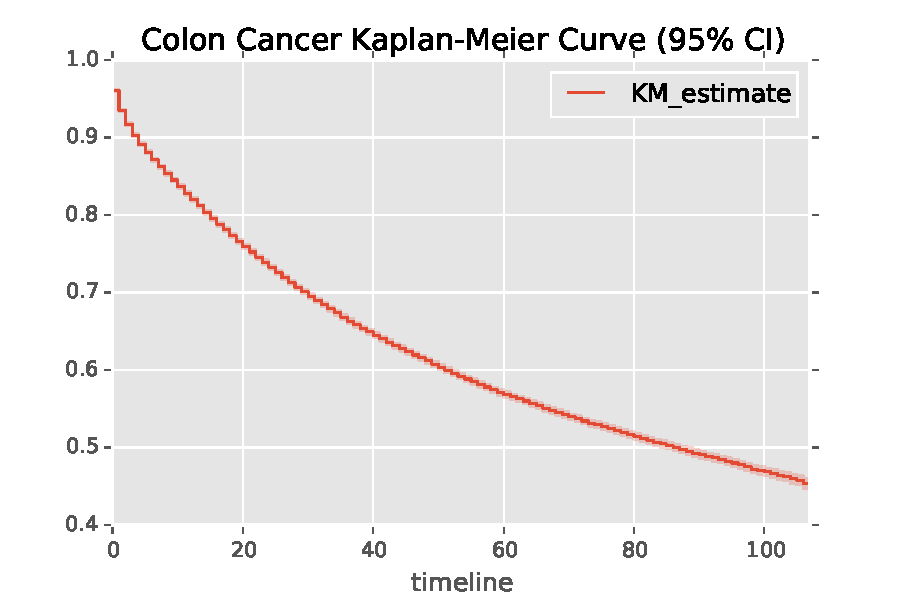
\includegraphics[width=.90\textwidth,origin=c]{colonkaplan.pdf}
% "\includegraphics" is very powerful; the graphicx package is already loaded
%\caption{\label{fig:colonkaplan} Traditional Kaplan-Meier estimate of the survival curve for all %colon cancer patients. Fitted with 113072 observations, 71804 censored.}
%\end{center}
%\end{figure}

%\begin{figure}[tbp]
%\centering 
%\begin{center}/\end{center} takes some additional vertical space
%\includegraphics[width=.45\textwidth,trim=0 380 0 200,clip]{img1.pdf}
%\hfill
%\begin{center}
%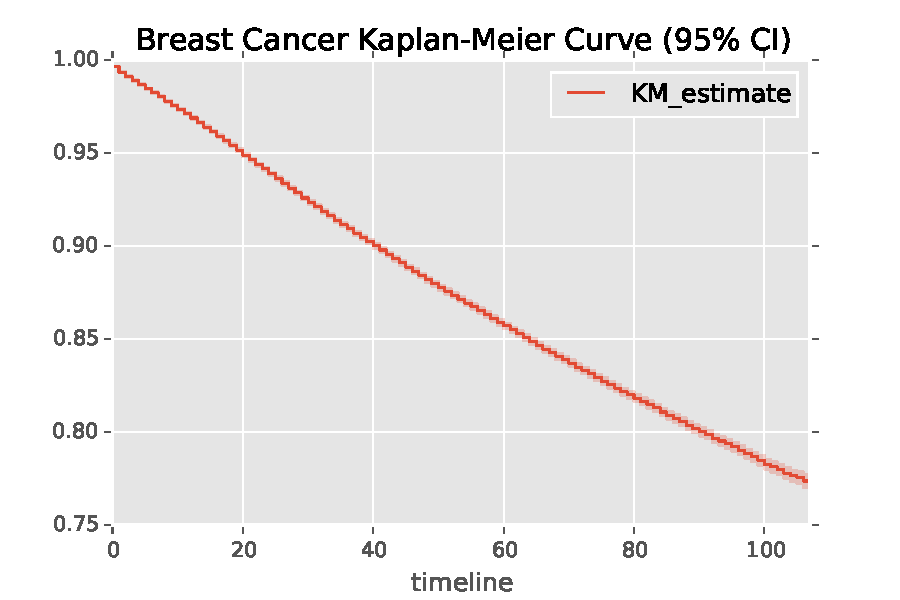
\includegraphics[width=.90\textwidth,origin=c]{breastkaplan.pdf}
% "\includegraphics" is very powerful; the graphicx package is already loaded
%\caption{\label{fig:breastkaplan} Traditional Kaplan-Meier estimate of the survival curve for all %breast cancer patients. Fitted with 329949 observatins, 292279 censored.}
%\end{center}
%\end{figure}


%\begin{figure}[tbp]
%\centering 
%\begin{center}/\end{center} takes some additional vertical space
%\includegraphics[width=.45\textwidth,trim=0 380 0 200,clip]{img1.pdf}
%\hfill
%\begin{center}
%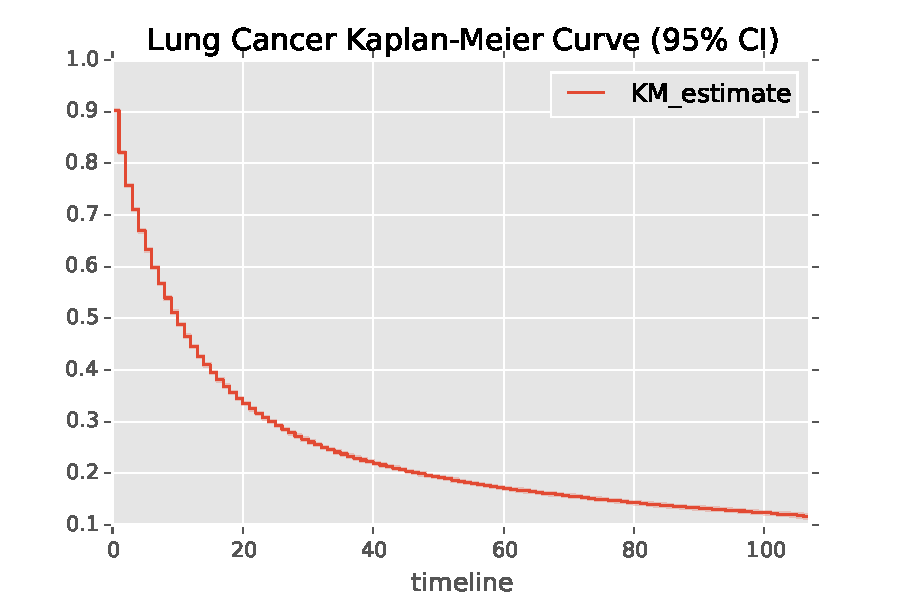
\includegraphics[width=.90\textwidth,origin=c]{lungkaplan.pdf}
% "\includegraphics" is very powerful; the graphicx package is already loaded
%\caption{\label{fig:lungkaplan} Traditional Kaplan-Meier estimate of the survival curve for all %lung cancer patients. Fitted with 177089 observatins, 47409 censored.}
%\end{center}
%\end{figure}


\subsection*{Transformation of Censored Data for Machine Learning}
\label{subsec:transformation}

In this section we describe an inuitive way to transform right-censored data appropriately so that it may be used as input to machine learning algorithms that learn the hazard fuction. The full details of this transformation, and a large inspiration for this study, can be flound in this blog post~\cite{kuhn}.



The overall philosophy of the Kaplan-Meier estimate of the survival curve for a population differs fundamentally from the methods described below and used in this study. 
The Kaplan-Meier estimate of the survival curve is given by
\begin{equation}
\label{eq:kaplanmeier}
\hat{S}(t) = \prod_{t_i < t} \frac{n_i - d_i}{n_i}
\end{equation}
where $d_i$ are the number of death events at time $t$ and $n_t$ is the number of subjects at risk of death just prior to time $t$. 
Equation~(\ref{eq:kaplanmeier}) uses the entire data set to arrive at an estimate of the entire population survival curve. In contrast, the method described below uses the entire data set to learn a model so as to predict hazard and survival curves from the data for as yet unseen individuals.


The key observation is to note that the hazard function can be directly learned via standard machine learning methods. It can be rewritten as
\begin{equation}
\label{eq:hhazard}
\lambda(\mathbf{X}, t) = P(Y = t|Y \geq t, \mathbf{X}),
\end{equation}
the probability that, if someone has survived up until month $t$, they will die in that month.
where $\mathbf{X}$ represents all of the data for that particular record, and in our case $Y$ represents the true, uncensored number of survival months of the patient.
What is actually provided in the SEER data is the related variable \codewhite{SURVIVAL MONTHS} $T$ (how long each subject was in the study), and whether they exited by dying or being censored ($D$), \codewhite{VITAL STATUS RECODE}. 
$D$ is a Boolean variable, so $D = 1$ if $T = Y$, and $D = 0$ if $T < Y$.



It follows directly from equation~\ref{eq:hhazard} that 
\begin{equation}
\label{eq:pmf}
P(Y = t | \mathbf{X}) = \lambda(\mathbf{X}, t) \prod_{i=1}^{t-1} (1 - \lambda(\mathbf{X}, i))
\end{equation},
which is the full probablity distribution of dying at time Y~\cite{kuhn}.
The survival function is then readily derived from this distribution as
\begin{equation}
\label{eq:cdf}
S(\mathbf{X},t_{k}) = 1 - CDF(\mathbf{X}, t_{k})
\end{equation}
where $CDF(\mathbf{X}, t_{k}) = \sum_
{k=1}^{n} P(Y = t_{k} | \mathbf{X}) $ is the cumulative density function correponding to the probability mass function in equation~\ref{eq:pmf}~\cite{downey}.




%In the discrete time variable case (which holds for the SEER data; \codewhite{SURVIVAL %MONTHS} takes on integer values), the relationship between the hazard function and the survival %function is given as follows~\cite{amstat}. Supppose that 
%$a_{j} < t \leq a_{j+1}$ where $a_{j}$ represents $j$ months. Then


%\begin{eqnarray}
%P(Y = t | \mathbf{X} ) & = & 


%\begin{eqnarray}
%S(t) &  = & P(T \geq a_{1}, T \geq a_{2}, \cdots , T \geq a_{j+1}) \\
%   & = & P(T \geq a_{1}) P(T \geq a_{2} | T \geq a_{1}) \cdots P(T \geq a_{j+1} | T \geq a_{j}) %\\
% & = & (1 - \lambda_{1}) \times \cdots \times (1 - \lambda_{j}) \\
% & = & \prod_{k: a_{k} < t}(1 - \lambda_{k}) \label{eq:hazardtosurvival}
%\end{eqnarray}



Treating $T$ as just another covariate is the key to the transformation. Each datapoint in the hidden classification problem is the combination of an $\mathbf{X}_{i}$ in the orginal dataset plus some month $t$, and the classification problem is "did point $\mathbf{X}_{i}$ die in month $t$.'' We will call this new variable $D_{it}$ (\codewhite{newtarget}).
We can transform our original data set into a new one, with one row for each month that each $\mathbf{X}_{i}$ is in the sample; train a standard classifier on this new dataset with $D_{it}$ as the target, and derive a survival model from the orginal dataset.
Psuedocode for this transformation is found in section~\nameref{subsec:pseudocode}.

Explicit examples will help make this transformation clear.
The untransformed datapoint represented Table~(\ref{tab:originaldead}) is transformed to the multiple records shown in Table~(\ref{tab:transformeddead}). All uncensored data is transformed in this way. All censored data is similarly transformed. 
The untransformed datapoint represented Table~(\ref{tab:originalalive}) is transformed to the multiple records shown in Table~(\ref{tab:transformedalive}).



\begin{table}[!ht]
\begin{adjustwidth}{-2.25in}{0in} % Comment out/remove adjustwidth environment if table fits in text column.
\caption{\label{tab:originaldead} {\bf Example of four columns in an uncensored record in the untransformed dataset.}}
\rowcolors{1}{white}{light-gray}
\begin{tabular}{lrrrr}
\toprule
{} &  \codewhite{cs\_tumor\_size} &  \codewhite{year\_of\_birth} &  \codewhite{survival\_months} &  \codewhite{vital\_status\_recode\_Dead} \\
\midrule
newindex &                &                &        &            \\
205      &             60 &           1951 &      3 &          1 \\
\bottomrule
\end{tabular}
\end{adjustwidth}
\end{table}



\begin{table}[!ht]
\begin{adjustwidth}{-2.25in}{0in} % Comment out/remove adjustwidth environment if table fits in text column.
\caption{\label{tab:originalalive} {\bf Example of four columns in a censored record in the untransformed dataset.}}
\rowcolors{1}{white}{light-gray}
\begin{tabular}{lrrrr}
\toprule
{} &  \codewhite{cs\_tumor\_size} &  \codewhite{year\_of\_birth} &  \codewhite{survival\_months} &  \codewhite{vital\_status\_recode\_Dead} \\
\midrule
newindex &                &                &        &            \\
205      &             40 &           1950 &      3 &          0 \\
\bottomrule
\end{tabular}
\end{adjustwidth}
\end{table}


\begin{table}[!ht]
\begin{adjustwidth}{-2.25in}{0in} % Comment out/remove adjustwidth environment if table fits in text column.
\caption{\label{tab:transformeddead} {\bf Example of four columns in an uncensored record in the transformed dataset.}}
\rowcolors{1}{white}{light-gray}
\begin{tabular}{lrrrr}
\toprule
{} &  \codewhite{cs\_tumor\_size} &  \codewhite{year\_of\_birth} &  \codewhite{month} &  \codewhite{newtarget} \\
\midrule
newindex &                &                &        &            \\
205      &             60 &           1951 &      0 &          0 \\
205      &             60 &           1951 &      1 &          0 \\
205      &             60 &           1951 &      2 &          0 \\
205      &             60 &           1951 &      3 &          1 \\
\bottomrule
\end{tabular}
\end{adjustwidth}
\end{table}


\begin{table}[tbp]
\begin{adjustwidth}{-2.25in}{0in} % Comment out/remove adjustwidth environment if table fits in text column.
\caption{\label{tab:transformedalive} {\bf Example of four columns in a censored record in the transformed dataset.}}
\rowcolors{1}{white}{light-gray}
\begin{tabular}{lrrrr}
\toprule
{} &  \codewhite{cs\_tumor\_size} &  \codewhite{year\_of\_birth} &  \codewhite{month} &  \codewhite{newtarget} \\
\midrule
newindex &                &                &        &            \\
205      &             40 &           1950 &      0 &          0 \\
205      &             40 &           1950 &      1 &          0 \\
205      &             40 &           1950 &      2 &          0 \\
205      &             40 &           1950 &      3 &          0 \\
\bottomrule
\end{tabular}
\end{adjustwidth}
\end{table}



One obvious side effect of this transformation is that it explodes the length of the dataset.
For this study, the original, untransformed colon cancer DataFrame has shape $(113072, 103)$, and the total transformed colon cancer DataFrame has shape $(4165251, 103)$.
Similary, the original, untransformed lung cancer DataFrame has shape $(177089, 115)$, and the total transformed lung cancer DataFrame has shape $(3079931, 115)$.
The biggest explosion in dataset size occured with the breast cancer data, which is a consequence of the relatively high survival rates in breast cancer. A subject who is censored with a recorded survival months of 48 will contribute an extra 48 rows to the transformed dataset.  
The original, untransformed breast cancer DataFrame has shape $(329949, 67)$, and the total transformed breast cancer DataFrame has shape $(15085711, 67)$.
Traning machine learning algorithms on such large datasets, even after splitting into training and testing sets described below, require large RAM. All computations for this study were performed on a Dell XPS 8700 Desktop with 32GB of RAM.

\subsection*{Training and Test Partitions}
\label{subsec:traintest}


After performing the data transformation adumbrated above, it is necessary to be mindful of how we partition the data into training and testing data. Each subject that was represented by a single row in the original untransformed dataset now potentially is represented by multiple rows in the transformed dataset, and care must be taken to ensure that all of the rows corresponding to a particular subject are either assigned exclusively to the training set or exclusive to the testing set. 
An additional characteristic of this transformed data that requires careful treatment involves balancing. The transformation results in many new records with the target variable \codewhite{newtarget} == 0. The training and test sets must be chosen such that the ratio of the number of records with \codewhite{newtarget} == 0 to that of the number of records with \codewhite{newtarget} == 1 is the same in the training and test datasets.
This ratio turns out to be $\approx 396$ for the breast cancer data, $\approx  99$ for the colon cancer data, and 
$\approx 22.75$ for the lung cancer data. 
The shapes of the training and testing datasets for breast cancer used in this study are $(14936862, 67)$ and 
$(148849, 67)$, respectively.
For lung cancer, the corresponding datasets have shapes $(2988768, 115)$ and $(91163, 115)$.
Finallly, for colon cancer the partition into training and test datasets of the transformed data have the shapes 
$(3958008, 103)$ and $(207243, 103)$. Multiple rows correspond to the same test patient in these datasets.
The colon cancer test dataset represents 5654 distinct subjects; the breast cancer test dataset represents 3300 distinct subjects; and the lung test dataset contains data for 5313 distinct subjects.

The models described below are trained to learn the values of \codewhite{newtarget}, which is a binary variable: a value of '0' indicating that the subject is still alive at the given month, while a value of '1' indicates that the patient died at that particular value of \codewhite{months}. The random forests and neural networks described below are binary classifiers with the target \codewhite{newtarget}. Fortunately, both the random forests and neural networks are capable of not only performing strict class prediction, i.e. predicting whether \codewhite{newtarget} is '0' or '1', but are also able to predict the \textit{probability} of \codewhite{newtarget} being '0' or '1'., and thus learning the hazard function.


Finally, we emphasize the crucial point that the features \codewhite{survival\_months} and \\
\codewhite{vital\_status\_recode\_Dead} are dropped from both the training and and testing data, and are replaced with the features \codewhite{months} and \codewhite{newtarget}, as illustrated in Tables~(\ref{tab:originaldead},~\ref{tab:originalalive},~\ref{tab:transformeddead},~\ref{tab:transformedalive}). The information of which subjects represent censored data (\codewhite{vital\_status\_recode\_Dead} == 0) and which died is retained and recoverable trough the \codewhite{newindex} variable and is needed for proper evaluation of the performance metrics; when evaluating AUC curves for the 6, 12, and 60 month binary classifiers, we need to limit the test data to those subjects that we know definitively whether or not they survived 6, 12 or 60 months respectively. This requirement will necessitate the elmination of some of the censored data when computing some of the performance metrics. We introduce the two machine learning algorithms used in this study below, chosen because of their high performance in machine learning competitions and their complementary methods, so that their mutual agreement shown below on the test datasets can be taken as indication that they are actually learning useful information.


Random Forests are made up of an ensemble of independent \textbf{Decision trees} that are purposefully exposed to only subsets of the data. The general philosophy is presented in the popular science book "The Wisdom of Crowds''~\cite{wisdom}.
The idea is that a large number of independent non-expert opinions converge on the correct answer when averaged. The success of this philosophy of prediction was startingly shown by the success of the political and world event predictions made by the prediction market site Intrade, before its forced closure by the Commodity Futures Trading Commission~\cite{cassidy}. %\footnote{``What killed Intrade?``, John Cassidy, \textit{The New Yorker}, 10 Mar, 2013, %accessed 11 Jan 2016, \url{http://www.newyorker.com/news/john-cassidy/what-killed-%intrade}.} 
 The other class of methods used by IOBS to develop predictive models are called neural networks, and are modelled on how the human brain learns high level concepts from lower level ones. 
As opposed to the crowd-based wisdom of a random forest, a neural network is analgous to a seasoned expert. 
%The philosophy behind the training and achieved accuracies of neural network classifiers and %predictors is that of going to a seasoned expert. 
A Neural network learns from repeated exposure to the training data and improves its predictions with each pass over the data.
 The general philosophy is simlar to that represented by the well-known maxim that it takes 10,000 hours to become an expert in any given field~\cite{outliers}.
%\footnote{``The 10,000 Hour Rule,` Malcolm Gladwell, accessed 11 Jan 2016, \url{http://%gladwell.com/outliers/the-10000-hour-rule/}.}


\subsection*{Prediction Models}
\label{sec:predmodels}

With the datasets transformed as described above, we are now able to use them to train and evaluate machine learning classifiers.
The classifier models described in this section are learning the hazard function: given all of the data given in the Supporting Information section for each cancer type and includes the field \codewhite{months} (the months after diagnosis), the models predict the target variable \codewhite{newtarget}, which is a binary class label equal to 1 if the subject died in that month and 0 otherwise.
Fortunately, both random forests and neural networks are capable of not only performing strict class prediction, i.e. predicing whether \codewhite{newtarget} is 0 or 1, but are also able to predict the \emph{probability} of \codewhite{newtarget} being 0 or 1, and thus learning the hazard function.
%Both random forests and neural networks can be used not only as binary classifiers, but also have the ability to predict %the \emph{probabilities} of belonging to either class encoded by \codewhite{newtarget}. In particular, the predicted %probability 
%of belonging to class 1 is exactly the hazard function corresponding to that value of \codewhite{months}: the probability %of dying in that month,
%, given that the patient represented by the record has survived up to that month. 
The models learn $\lambda(\mathbf{X}, \codewhite{months})$.
This prediction task should not be confused with the regression problem of trying to predict precisely in what month a patient will die.


The hazard functions thus learned and predicted are intermediary products; what we are really pursuing are the survival functions for each patient that are derived from the predicted hazard functions.
From the resulting hazard functions for each unique patient, we can construct the
resulting survival functions as presented in section~(\ref{subsec:pseudocode}) and Equation~(\ref{eq:hazardtosurvival}) and explicitly given in python code in the notebooks at the github repository containing supplemental material for this study~\cite{supp}.
For each subject $i$, all input data minus \codewhite{months} and \codewhite{newtarget} is represented by $\mathbf{X}_{i}$. After the classfier models have trained with target \codewhite{newtarget} on the (very large) training set, each subject's survival function is computed in the corresponding (much smaller) test set.
These functions are computed by using the model to predict $\lambda(\mathbf{X}_i, t_{j})$ for $j$ running from 0 to 107 months, and $\mathbf{X}_{i}$ corresponds to the single row corresponding to subject $i$ in the original untransformed dataset.
107 months was the maximum value of survival months in all three of the cancer datasets, and is a consequence of the data subsets chosen for this study.

\paragraph{Decision Trees and Random Forests}
\emph{Decision tree} classifiers are attractive models because they can be intrepeted easily. Like the name decision tree suggests, we can think of this model as breaking down our data by making decisions based on asking a series of questions.
Based on the features in our training set, the decision tree model learns a series of questions to infer the class labels of the samples. 

\emph{Random forests} have gained huge popularity in applications of machine learning during the last decade due to their good classification performance, scalability, and ease of use. Intuitively, a random forest can be considered as an \emph{ensemble of decision trees}. The idea behind ensemble learning is to combine \emph{weak learners} to build a more robust model, a \emph{strong learner}, that has a better generalization error and is less susceptible to overfitting. 

The goal behind \emph{ensemble methods} is to combine different classifiers into a meta-classifier that has a better generalization performance than each individual classifier alone. For example, assuming that we collected predictions from 10 experts, ensemble methods would allow us to strategically combine these predictions by the 10 experts to come up with a prediction that is more accurate and robust than the predictions by each individual expert. The individual decision trees that make an ensemble are called base learners, and as long as the error rate of each base learner is less than .50, the combined random forest will benefit from the affects of combining predictions to achieve a far greater accuracy.

Figure~(\ref{fig:ensemble}) illustrates the power of ensemble methods; the Figure illustrates how the ensemble error rate is much lower than the Base learner error rate, as long as the Base learner error rate is less than 0.5. The Figure illustrates this effect for an ensemble of 500 base learners.



\begin{figure}[!ht]
  \centering
    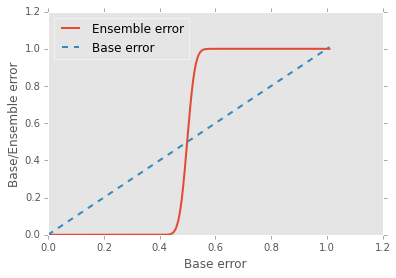
\includegraphics[scale=.75]{ensemble}
\caption{\label{fig:ensemble} Illustration of ensemble methods showing how a collection of base learners with poor accuracy can combine to produce an accurate ensemble learner.}
\end{figure}


A big advantage of random forests is that honing in on suitable hyperparameter values (the number of trees in the forest, the depth of each decision tree, the specific measure of information gain used to choose the node splitting, etc) is not very difficult. The ensemble method is robust to noise from the individual decision trees, which helps to prevent overfitting (memorizing the training dataset targets instead of generalizing from learned rules to perform successfuly on unseen data). The only parameter that has a clearly noticeable effect on performance is the number of trees to include in the forest; in general, the more trees the better the performance, but there is a price to pay in terms of computational cost. The number of trees for the forests trained in this study was relatively small, 20 trees for breast cancer and 25 for both the lung and colon cancer models. 

IOBS has chosen to use the Python scikit-learn implemenation of the Random Forest machine 
learning classifier~\cite{rf}.
Random Forests are frequent winners of the Kaggle machine learning competitions~\cite{kagglerf}.
The model parameters for each cancer type are given in sections~(\nameref{subsec:lungrf},~\nameref{subsec:colonrf},~\nameref{subsec:breastrf}).


\paragraph{Multi-Layer Perceptron Neural Networks}
Neural networks are a biologically-inspired programming paradigm that enable computers to learn from observational data~\cite{deeplearning}.
%As you may know, \textbf{deep learning} is getting a lot of press and is without any doubt the %hottest topic in the machine learning field.
Deep learning can be understood as a set of algorithms that were developed to train artificial neural networks with many layers most efficiently.
 Neural networks are a hot topic not only in academic research, but also in big technology companies such as Facebook, Microsoft, and Google who invest heavily in artificial neural networks and deep learning research. As of today, complex neural networks powered by deep learning algorithms are considered as state-of-the-art when it comes to complex problem solving such as image and voice recognition.
In addition, the pharmaceutical industry recently started to use deep learning techniques for drug discovery and toxicity prediction, and research has shown that these novel techniques substantially exceed the performance of traditional methods for virtual screening~\cite{toxicity}.

IOBS has chosen to use the Multi-Layer Perceptron Neural Network (MLP neural network) implementation Keras developed at MIT.
Keras was initially developed as part of the research effort of project ONEIROS (Open-ended Neuro-Electronic Intelligent Robot Operating System)~\cite{keras}.
Keras is a minimalist, highly modular neural networks library, written in Python and capable of running on top of either TensorFlow or Theano. The model architecture for each cancer type are given in sections~(\nameref{subsec:breastnn},~\nameref{subsec:colonnn},~\nameref{subsec:lungnn}). Training a neural network and choosing an appropriate architecture is as much art as science~\cite{deeplearning}, and the search for a good neural network architecture for the lung cancer case was more demanding than for the breast and colon cases. The presence of both non-small cell lung cancer (NSCLC) and small cell lung cancer (SCLC) in the SEER data may be the source of this need for more iterations and trials of different architectures when training the lung cancer neural network models.




%\subsection*{Etiam eget sapien nibh.}

% For figure citations, please use "Fig." instead of "Figure".
%Nulla mi mi, Fig.~\ref{fig1} venenatis sed ipsum varius, volutpat euismod diam. Proin rutrum %vel massa non gravida. Quisque tempor sem et dignissim rutrum. Lorem ipsum dolor sit amet, %consectetur adipiscing elit. Morbi at justo vitae nulla elementum commodo eu id massa. In %vitae diam ac augue semper tincidunt eu ut eros. Fusce fringilla erat porttitor lectus cursus, %%\nameref{S1_Video} vel sagittis arcu lobortis. Aliquam in enim semper, aliquam massa id, %cursus neque. Praesent faucibus semper libero.

%\begin{figure}[h]
%\caption{{\bf Figure Title first bold sentence Nulla mi mi, venenatis sed ipsum varius, volutpat %euismod diam.}
%Figure Caption Proin rutrum vel massa non gravida. Quisque tempor sem et dignissim rutrum. %A: Lorem ipsum dolor sit amet. B: Consectetur adipiscing elit.}
%\label{fig1}
%\end{figure}

%\begin{enumerate}
%\item{react}
%\item{diffuse free particles}
%\item{increment time by dt and go to 1}
%\end{enumerate}

% Results and Discussion can be combined.
\section*{Results}
\label{sec:results}


In order to evaluate the performance of the models, we first construct three binary classifiers corresponding to whether or not a subject survived 6, 12, or 60 months after diagnosis. 
This is done by iterating over all distinct patient indices in the test set, prediciting the full survival function, and capturing the values corresonding to 6, 12, and 60 months.  
If the survival function evaluted at 6 months is greater than or equal to .5 for a given subject, then the 6 months binary classifier predicts that that subject will be alive 6 months after diagnosis. Similarly, if the survival function evaluted at 60 months is less than .5, then the 12 months binary classifier predicts that that subject will be dead 12 months after diagnosis. Figure~(\ref{fig:survivalexample}) illustrates the method; in this case the 6-month and 12-month classifiers predict survival, while the 60-month classifier predicts expiry.


%\begin{figure}[tbp]
\begin{figure}[h]
\centering 
%\begin{center}/\end{center} takes some additional vertical space
%\includegraphics[width=.45\textwidth,trim=0 380 0 200,clip]{img1.pdf}
%\hfill
\begin{center}
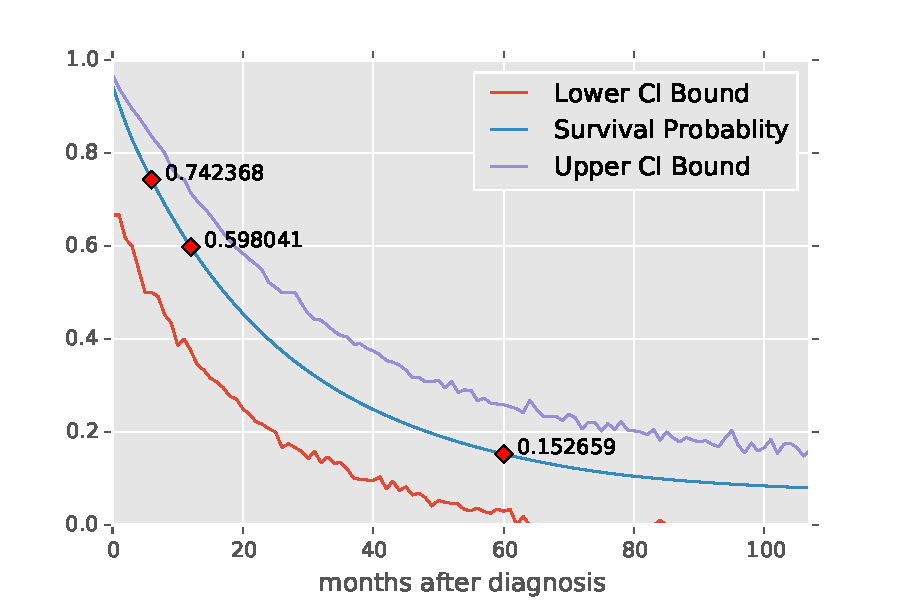
\includegraphics[width=.90\textwidth,origin=c]{survivalexamplewitherrors.pdf}
% "\includegraphics" is very powerful; the graphicx package is already loaded
\caption{\label{fig:survivalexample} Example of the construction of the binary classifiers for 6, 12, and 60 months survival.
A subject's hazard curve $\lambda(\mathbf{X}, t)$ is predicted by the model for times out to 107 months. The survival curve is then readily computed as in Equation~(\ref{eq:cdf}). For this example, the 6-month and 12-month classifiers predict survival, while the 60-month classifier predicts expiry.}
\end{center}
\end{figure}



Because of censoring it is necessary to apply some Boolean filters to the data in order to correctly assess the resulting classifiers.
To construct AUC curves for the 6 month classifier, we restrict ourselves to considering
subjects in the test data where either of the following mutually exlusive conditions holds:

\begin{itemize}[noitemsep]
\item \codewhite{survival\_months} $>=$ 6 AND \codewhite{vital\_status\_recode} == 0
\item \codewhite{vital\_status\_recode} == 1
\end{itemize}




That is, we restrict ourselves to subsets of the data where we know for certain whether or not the subject survived at least 6 months. Similarly for the 12 and 60 months surivival classifiers. 

\paragraph{Survival Curve Error Estimates}
The standard calculation of confidence intervals used in the Kaplan-Meier estimates of survival curves does not apply for these personal predictions. The following bootstrap method was used to calculate the upper and lower bounds corresponding to 95\% confidence intervals.
From equation~\ref{eq:cdf}, we can obtain the cumulative distribution function (CDF) associated with each individual survival curve.
We then sample from this CDF in a way that reflects the underlying data used to produce the model. The training data used to create the model has an underlying distribution of survival months. In the transformed training dataset, each subject contributes as many rows as the number of survival months plus one (patients with zero survival months still represent one row of the training data). A subject that survived 50 months contributes 51 "points" to the training of the model. If all patients lived out to 107 months, the model would contain less uncertainty. This observation leads to the following algorithm for determining the error estimates to the predicted survival curves:

\begin{itemize}[noitemsep]
\item compute the CDF associated with the survival curve
\item use the underlying training data CDF of survival months to choose the number of points
to draw from the survival curve CDF, and compute a new survival curve 
\item Repeat the previous step 10,000 times and collect the curves into a list. Changing the number of curves affects how smooth the upper and lower bounds are, but does not affect the interval size between for each month.
\item extract for each month from the list of curves the .975 and .025 percentiles to record the values for the upper and lower curves
\end{itemize}

The process is somewhat anologous to the following hypothetical situation. Imagine a patient going to an expert, and the expert after collecting data on the patient and keeping records predicts the central, single survival curve. The patient then seeks multiple "second opinions.'' These second opinions are generated not from independent examinations of the patient, but by outside experts sampling from the data already collected by the expert initially consulted. 
Then the predictions of 95\% of these 10,000 experts all fall within the band determined by the upper and lower curves.





\subsection*{Performance Metrics}
\label{sec:performancemetrics}



The AUC scores for each of the 18 different binary classifiers are listed in Table~(\ref{tab:AUC}). We emphasize the above-mentioned discussion concerning the correct treatment of the censored test data when evaluating performance metrics.
Namely, when computing the AUC for the 12 month survival curve classifiers, we restrict the test data subjects to those that in the untransformed data set that satisfy either of the following mutually exclusive conditions:



\begin{itemize}[noitemsep]
\item \codewhite{survival\_months} $>=$ 12 AND \codewhite{vital\_status\_recode} == 0
\item \codewhite{vivtal\_status\_recode} == 1
\end{itemize}

We limit evaluation data to subsets of the data where we know for certain whether or not the subject survived at least 12 months. Similar considerations apply to the 12 and 60 months AUC calculations. The lowest AUC in Table~\ref{tab:AUC} is .765, corresponding to the lung neural network model predictions for 6 months survival, while the highest AUC in Table~\ref{tab:AUC} is .885, corresponding to the breast random forest model predictions for 12 months survival.


\begin{table}[!ht]
\begin{adjustwidth}{-2.25in}{0in} % Comment out/remove adjustwidth environment if table fits in text column.
\caption{\label{tab:AUC} {\bf AUC values for the Random Forest and Neural Networks model
binary classifiers derived from the full survival curve predictions; see text for details. The number of subjects that were used in the calculation of a given AUC score are given in parenthesis after the score. }}
\rowcolors{1}{white}{light-gray}
\begin{tabular}{lrrr}
\toprule
%\rowcolors{1}{white}{yellow}
%\hline
Model & 6 Months AUC & 12 Months AUC & 60 Months AUC \\ 
\midrule
Breast RF &  .846  (3035)     &     .885  (2797)         &  .844 (1392) \\ 
Breast NN &   .855 (3035)    &     .867  (2797)    &    .836  (1392) \\ 
Colon RF  &     .804 (5281)         &      .806 (5003)          &      .828   (3232)        \\ 
Colon NN   &     .797 (5281)         &          .804 (5003)        &   .841 (3232) \\ 
Lung RF    &      .772  (5019)             &        .796 (4860)              &   .874 (4143)  \\ 
Lung NN    &        .765  (5019)            &        .796  (4860)             &  .875 (4143)  \\
\bottomrule
\end{tabular}
\end{adjustwidth}
\end{table}




\subsection*{Model Agreement}
\label{subsec:agreement}



An additional means of validating the predictions of these models is by comparing their predictions to each other for the same set of input data. 
Table~\ref{tab:agree} shows the strong agreement between the random forest and neural network classifiers for each cancer type. Python code showing how the values in Table~\ref{tab:agree} are computed is available in the files 
\codewhite{NewPatientBreastCF.html}, \codewhite{NewPatientColonCF.html}, and \codewhite{NewPatientLung.html} in the GitHub repository containing supplemental matierial for this study~\cite{supp}. Table~\ref{tab:agree} is computed as follows. 
For each cancer type (breast,colon, and lung), do the following:

\begin{itemize}[noitemsep]
\item use the corresponding Random Forest and Neural Network models to compute the survival curves for all of the test subjects
\item extract the values of the survival curve evaluted for 6, 12, and 60 months for both models
\item if both models predict less than .5 or both models predict greater than or equal to .5, that counts as agreement
\item otherwise, the models disagree
\end{itemize}


The high level of agreement between two models lends confidence to the notion that they have both learned from the training data and are generalizing well. Figures~(\ref{fig:colonbox},~\ref{fig:breastbox},~\ref{fig:lungbox}) 
show box plots of the value of the random forest prediction subtracted from the neural network prediction.
We emphasize that when evaluating the model agreement, we put no restrictions on the distinct subjects in the respective test datasets; we are confronting the models against each other, not some known ground truth as in the AUC performance metric calculations. The number of distinct subjects in all three of the colon cancer survival binary classifiers (6, 12, and 60 month survival) was 5654; for lung cancer the number of subjects entering into the calculation of Table~(\ref{tab:agree})
 was 5313; and for breast cancer it was 3300.


\begin{table}[!ht]
\begin{adjustwidth}{-2.25in}{0in} % Comment out/remove adjustwidth environment if table fits in text column.
\caption{\label{tab:agree} {\bf Percentage agreement for the Random Forest and Neural Network classifiers for 6, 12, and 60 month survival predictions on the test data for each cancer type.}}
\rowcolors{1}{white}{light-gray}
\begin{tabular}{lrrr}
\toprule
%\rowcolors{1}{white}{yellow}
Cancer Type & $\%$ agreement 6 months & $\%$ agreement 12 months & $\%$ agreement 60 months \\ 
\midrule
Colon & .981 & .971 & .915 \\  
Breast & .994 & .984 & .938 \\  
Lung & .861 & .883 & .900 \\  
\bottomrule
\end{tabular}
\end{adjustwidth}
\end{table}

\begin{figure}[tbp]
%\begin{figure}[H]
\centering 
%\begin{center}/\end{center} takes some additional vertical space
%\includegraphics[width=.45\textwidth,trim=0 380 0 200,clip]{img1.pdf}
%\hfill
\begin{center}
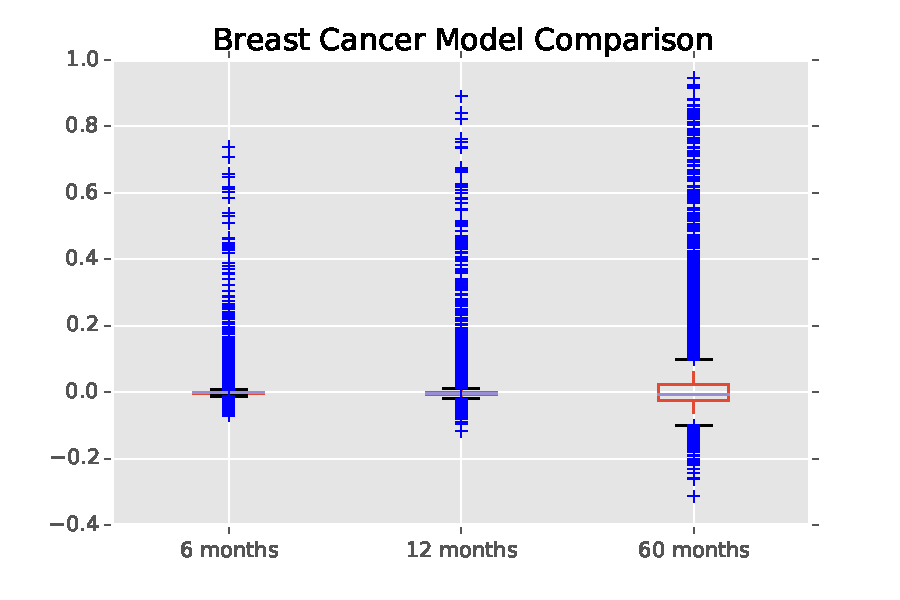
\includegraphics[width=.70\textwidth,origin=c]{breastbox.pdf}
% "\includegraphics" is very powerful; the graphicx package is already loaded
\caption{\label{fig:breastbox} Box plots showing the distributions of the signed difference between the MLP model's prediction for the probability of surviving 6 months and the Random Forest model's prediction of the same quantity for breast cancer. The plot shows the same quantity for the 12 and 60 months classifiers. It is apparent from the figures that the outliers are due to the neural network models predicting higher survival probablitlies than the random forest for some few cases. These differences were evaluated for the 3300 test patients in the breast cancer data.}
\end{center}
\end{figure}


\begin{figure}[tbp]
\centering 
%\begin{center}/\end{center} takes some additional vertical space
%\includegraphics[width=.45\textwidth,trim=0 380 0 200,clip]{img1.pdf}
%\hfill
\begin{center}
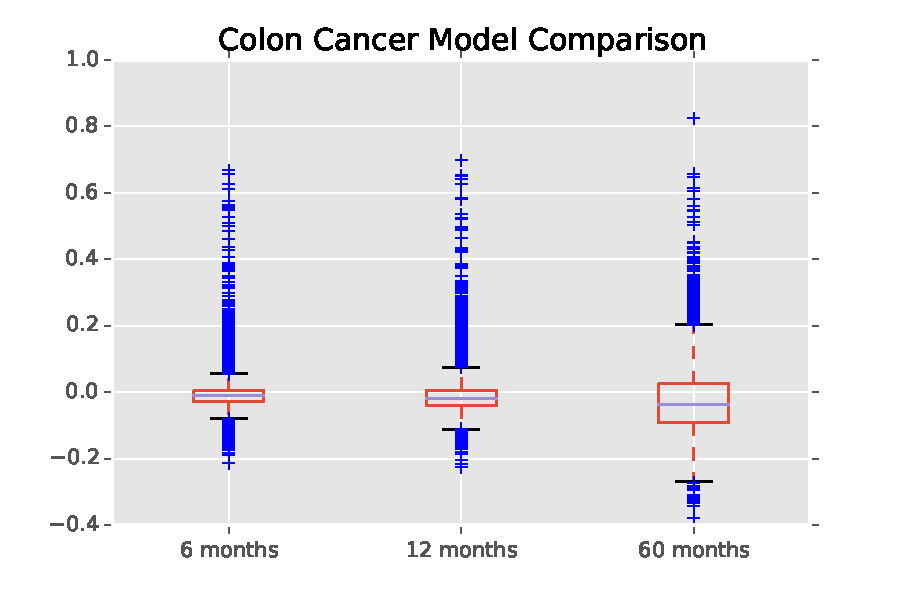
\includegraphics[width=.90\textwidth,origin=c]{colonbox.pdf}
% "\includegraphics" is very powerful; the graphicx package is already loaded
\caption{\label{fig:colonbox} Box plots showing the distributions of the signed difference between the MLP model's prediction for the probability of surviving 6 months and the Random Forest model's prediction of the same quantity for colon cancer. The plot shows the same quantity for the 12 and 60 months classifiers. It is apparent from the figures that the outliers are due to the neural network models predicting higher survival probablitlies than the random forest for some few cases. These differences were evaluated for the 5654 test patients in the colon cancer data.}
\end{center}
\end{figure}


\begin{figure}[tbp]
\centering 
%\begin{center}/\end{center} takes some additional vertical space
%\includegraphics[width=.45\textwidth,trim=0 380 0 200,clip]{img1.pdf}
%\hfill
\begin{center}
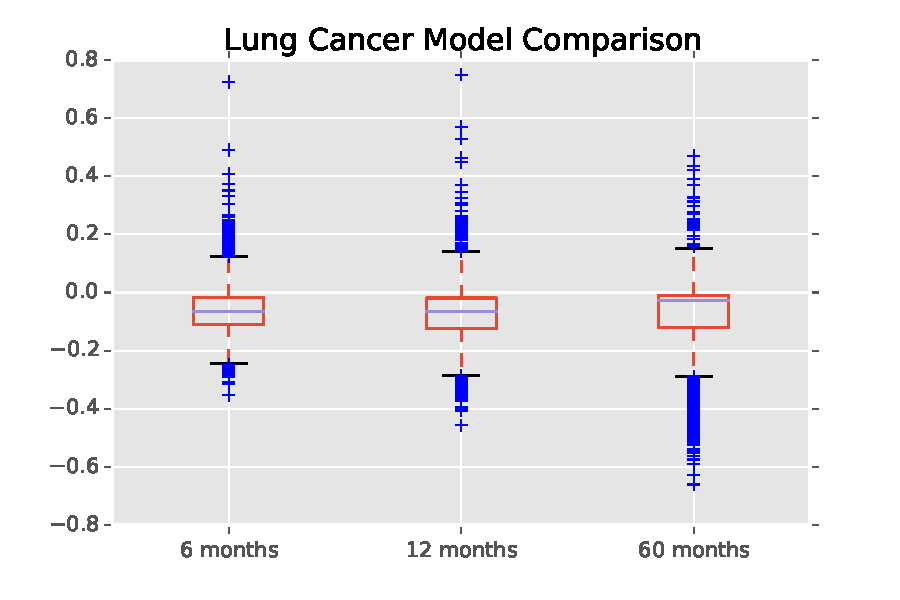
\includegraphics[width=.90\textwidth,origin=c]{lungbox.pdf}
% "\includegraphics" is very powerful; the graphicx package is already loaded
\caption{\label{fig:lungbox} Box plots showing the distributions of the signed difference between the MLP model's prediction for the probability of surviving 6 months and the Random Forest model's prediction of the same quantity for lung cancer. The plot shows the same quantity for the 12 and 60 months classifiers. These differences were evaluated for the 5313 test patients in the lung cancer data. The Interquartile Ranges for lung cancer are visibly larger than those for breast cancer and colon cancer shown in fig~\ref{fig:breastbox} and fig~\ref{fig:colonbox}.}
\end{center}
\end{figure}



\subsection*{Survival Curve Prediction Apps}
\label{sec:apps}


The six models described in section~\nameref{sec:predmodels}, namely the random forest and MLP neural network models for each of the three cancer types considered in this study, have their full hyperparameter and architecture presented in section~\nameref{sec:supporting}. Python code for all six model training and evaluation is available at the githib respository containing supplemental material for this study~\cite{supp}.



Using the popular Flask microframework for web applications~\cite{flask}, we have made web applications corresponding to the six models. The list of web applications below will allow readers to freely experiment with the models.

\begin{enumerate}[noitemsep]
\item breast cancer 
    \begin{enumerate}[noitemsep]
    \item random forest: \url{https://github.com/doolingdavid/breast-cancer-rf-errors.git}
    \item neural network: \url{https://github.com/doolingdavid/breast-cancer-nn-errors.git}
    \end{enumerate}
\item lung cancer
   \begin{enumerate}[noitemsep]
   \item random forest: \url{https://github.com/doolingdavid/lung-cancer-rf-errors.git}
   \item neural network: \url{https://github.com/doolingdavid/lung-cancer-nn-errors.git}
    \end{enumerate}
\item colon cancer
  \begin{enumerate}[noitemsep]
   \item random forest: \url{https://github.com/doolingdavid/colon-cancer-rf-errors.git}
   \item neural network: \url{https://github.com/doolingdavid/colon-cancer-nn-errors.git}
   \end{enumerate}
%\item prostate cancer
 % \begin{enumerate}[noitemsep]
%   \item random forest: \url{http://prostate-cancer.herokuapp.com/}
%   \end{enumerate}
\end{enumerate}

After downloading the .zip file associate with one of the above web applications, and assuming 
python is installed on your system, you can launch the application by running
\begin{verbatim}
>python hello.py
\end{verbatim}
and pointing the browser to the local server: \codewhite{http://127.0.0.1:5000}.


These machine learning models are used to predict survival curves for a given set of input data. 
The resulting surival curves predict the probablitiy that a patient with the given input data will survive at least up to month $x$.

 For example, using the Colon Cancer neural network app, and 
inputing the values listed in Table~(\ref{tab:boston1940}) results in the survival curve depicted in Figure~(\ref{fig:boston1940}); the predicted probablities of living 
at least 6, 12, and 60 months are .89, .83, and .50, respectively.



\begin{table}[!ht]
\begin{adjustwidth}{-2.25in}{0in} % Comment out/remove adjustwidth environment if table %fits in text column.
\caption{\bf{Example input data to the Colon Cancer neural network app \url{https://github.com/doolingdavid/colon-cancer-nn-errors.git}.}}
\rowcolors{1}{white}{light-gray}
\begin{tabular}{lr}
\toprule
  Variable  & Value \\ 
\midrule
  What is the tumor size (mm) & 300 \\  
  What is the patient's address? & boston massachusetts \\ 
  Grade & moderately differentiated \\  
  Histology & adenomas and adenocarcinomas \\ 
  Laterality & not a paired site \\  
 Martial Status at Dx & Single, never married \\  
 Month of Diagnosis & Jan \\  
 How many primaries & 1 \\  
  Race$\_$ethnicity & White \\  
  seer$\_$historic$\_$stage$\_$a  & Regional \\ 
  Gender & Male \\  
  spanish$\_$hispanic$\_$origin & Non-spanish/Non-hispanic \\ 
 Year of Birth & 1940 \\  
  Year of Diagnosis & 2010 \\
\bottomrule
\end{tabular}
\label{tab:boston1940}
\end{adjustwidth}
\end{table}


\begin{figure}[!ht]
%\caption{Colon Cancer Survival Curve.}
%  \label{fig:boston1940}
  \centering
    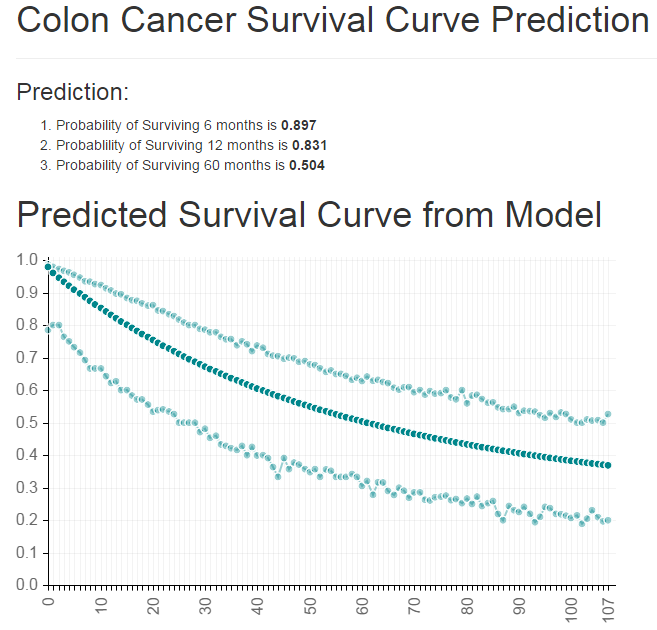
\includegraphics[scale=.8]{boston1940}
\caption{\label{fig:boston1940} Colon Cancer Survival Curve predicted from the data in 
Table~(\ref{tab:boston1940}) using the neural network web app \url{https://github.com/doolingdavid/colon-cancer-nn-errors.git}.}
\end{figure}

Changing the data in Table~\ref{tab:boston1940} so that the address field is changed from Boston, Massachusetts to Denver, Colorado but keeping all other variables are unchanged results in the predicted probabilities of living at least 6, 12, and 60 months: .945, .902, .665. 
Behind the scenes, the apps use the input to the address field to make a call to the Google Maps API to convert the address into a latitude, longitude and elevation.
These probablities are noticeably higher and reflect the documented effects of both longitude and elevation on cancer treatment and prognosis in the United States~\cite{kob4}.

A similar example of how changing the inputs to the models affects the predicted survival curves in interesting ways can be seen with the random forest model for lung cancer. Changing the data in Table~\ref{tab:lungmaritalstatus} by toggling between the male/female, and married/single four possible permutations results in the following prediction probabilites for 6, 12, and 60 month survival:

\begin{itemize}[noitemsep]
\item male/married:  .53, .27, .01
\item male/single: .35, .18, .009
\item female/married:  .55, .31, .01
\item female/single: .50, .27, .01
\end{itemize}


\begin{table}[!ht]
\begin{adjustwidth}{-2.25in}{0in} % Comment out/remove adjustwidth environment if table %fits in text column.
\caption{{\bf Example input data to the Lung Cancer random forest app \url{https://github.com/doolingdavid/lung-cancer-rf-errors.git}.}}
\rowcolors{1}{white}{light-gray}
\begin{tabular}{lr}
\toprule
  Variable  & Value \\ 
\midrule
  What is the tumor size (mm) & 500 \\  
  What is the patient's address? & newark new jersey \\ 
  Grade & well differentiated \\  
  Histology & acinar cell neoplasms \\ 
  Laterality & \makecell{bilateral involvement, lateral origin unknown; \\ stated to be single primary} \\  
 Martial Status at Dx & Married including common law \\  
 Month of Diagnosis & Jan \\  
 How many primaries & 1 \\  
  Race$\_$ethnicity & White \\  
  seer$\_$historic$\_$stage$\_$a  & Distant \\ 
  Gender & Female \\  
  spanish$\_$hispanic$\_$origin & Non-spanish/Non-hispanic \\ 
 Year of Birth & 1970 \\  
  Year of Diagnosis & 2011 \\
\bottomrule
\end{tabular}
\label{tab:lungmaritalstatus}
\end{adjustwidth}
\end{table}



Inputting the same combinations of data into the lung cancer neural network app \url{https://github.com/doolingdavid/lung-cancer-nn-errors.git}
yields the following probabilities:

\begin{itemize}[noitemsep]
\item male/married: .42, .24, .04
\item male/single: .40, .22, .03
\item female/married: .44, .26, .04
\item female/single: .42, .24, .04
\end{itemize}

It it interesting to note that both the random forest and neural network lung cancer models predict greater 6 month survival rates for married people, with a slightly greater benefit for males than females. The effect is greater in the random forest model, but is also visible in the neural network model. 

%\begin{table}[!ht]
%\begin{adjustwidth}{-2.25in}{0in} % Comment out/remove adjustwidth environment if table %fits in text column.
%\caption{
%{\bf Table caption Nulla mi mi, venenatis sed ipsum varius, volutpat euismod diam.}}
%\begin{tabular}{|l|l|l|l|l|l|l|l|}
%\hline
%\multicolumn{4}{|l|}{\bf Heading1} & \multicolumn{4}{|l|}{\bf Heading2}\\ \hline
%$cell1 row1$ & cell2 row 1 & cell3 row 1 & cell4 row 1 & cell5 row 1 & cell6 row 1 & cell7 row 1 %& cell8 row 1\\ \hline
%$cell1 row2$ & cell2 row 2 & cell3 row 2 & cell4 row 2 & cell5 row 2 & cell6 row 2 & cell7 row 2 %& cell8 row 2\\ \hline
%$cell1 row3$ & cell2 row 3 & cell3 row 3 & cell4 row 3 & cell5 row 3 & cell6 row 3 & cell7 row 3 %& cell8 row 3\\ \hline
%\end{tabular}
%\begin{flushleft} Table notes Phasellus venenatis, tortor nec vestibulum mattis, massa tortor %interdum felis, nec pellentesque metus tortor nec nisl. Ut ornare mauris tellus, vel dapibus arcu %suscipit sed.
%\end{flushleft}
%\label{table1}
%\end{adjustwidth}
%\end{table}



%\subsection*{\lorem\ and \ipsum\ Nunc blandit a tortor.}

%Maecenas convallis mauris sit amet sem ultrices gravida. Etiam eget sapien nibh. Sed ac ipsum %eget enim egestas ullamcorper nec euismod ligula. Curabitur fringilla pulvinar lectus %consectetur pellentesque. Quisque augue sem, tincidunt sit amet feugiat eget, ullamcorper sed %velit. Sed non aliquet felis. Lorem ipsum dolor sit amet, consectetur adipiscing elit. Mauris %commodo justo ac dui pretium imperdiet. Sed suscipit iaculis mi at feugiat. 

%\subsection*{Sed ac quam id nisi malesuada congue.}

%Nulla mi mi, venenatis sed ipsum varius, volutpat euismod diam. Proin rutrum vel massa non %gravida. Quisque tempor sem et dignissim rutrum. Lorem ipsum dolor sit amet, consectetur %adipiscing elit. Morbi at justo vitae nulla elementum commodo eu id massa. In vitae diam ac %augue semper tincidunt eu ut eros. Fusce fringilla erat porttitor lectus cursus, vel sagittis arcu %lobortis. Aliquam in enim semper, aliquam massa id, cursus neque. Praesent faucibus semper %libero.

% Please do not create a heading level below \subsection. For 3rd level headings, use %%\paragraph{}. 
%\subsection*{Subsection 1}
%Nulla mi mi, venenatis sed ipsum varius, volutpat euismod diam. Proin rutrum vel massa non %gravida. Quisque tempor sem et dignissim rutrum. Lorem ipsum dolor sit amet, consectetur %adipiscing elit. Morbi at justo vitae nulla elementum commodo eu id massa. In vitae diam ac %augue semper tincidunt eu ut eros. Fusce fringilla erat porttitor lectus cursus, vel sagittis arcu %lobortis. Aliquam in enim semper, aliquam massa id, cursus neque. Praesent faucibus semper %libero.

%\subsection*{Subsection 2}
%\paragraph{3rd Level Heading.} Nulla mi mi, venenatis sed ipsum varius, volutpat euismod %diam. Proin rutrum vel massa non gravida. Quisque tempor sem et dignissim rutrum. Lorem %ipsum dolor sit amet, consectetur adipiscing elit. Morbi at justo vitae nulla elementum %commodo eu id massa. In vitae diam ac augue semper tincidunt eu ut eros. Fusce fringilla erat %porttitor lectus cursus, vel sagittis arcu lobortis. Aliquam in enim semper, aliquam massa id, %cursus neque. Praesent faucibus semper libero.

\section*{Discussion}
\label{sec:discussion}


The purpose of this study has been twofold; to develop a general methodology of data transformation to survival data with censored observations so that machine learning algorithms can be applied and to help further the cause of PPPM medicine by developing models of personalized suvival curve prognosis.
To help further refine the methodology, we would like to apply it to different survival datasets~\cite{umass}, not necessarily within the healthcare domain. In particular, the methods presented in this paper do not take into account time varying features. For example, the \codewhite{cs\_tumor\_ size} variable that has been a part of this study is kept fixed at the value measured at diagnosis for all records corresponding to a given subject. Clearly, the actual tumor size varies along with time and a sophisitcated model can be developed to take this into account, given available datasets. Unfortunately, the SEER datasets considered in this study do not provide this kind of granularity over time.


The SEER database has been linked with claims data in the SEER-Medicare Linked Database~\cite{seermed}. This linkage allows for the identification of additional clinical data for each record in the SEER database and allows for an enrichment of the models presented in this study, and is an avenue for further investigation.


An additional avenue of research concerns the broad concept of causality. As demonstrated in section~\nameref{sec:apps}, there appears to be a correlation between marital status and survival prognosis. Does this mean that if a single person in Boston, Massachusetts is diagnosed with cancer, that they should immediately get married and move to Denver? Of course not. 
But personal discussions with providers has confirmed for one of the authors (D.D.) that married males tend to be much more diligent in following instructions than their single counterparts. What appears to be in effect is that some of the SEER data is providing an identifiable signature of underlying causes not directly represented by the data. Latent variables not directly seen in the data are still providing echos of patterns in the data and the sheer volume allows us to see glimpses of these patterns. Marital status is in some instances a surrogate for the presence of a strong social structure and support group surrounding a patient, which presence presumably leads to more desirable survival prognosis. 
The daunting and exciting task of teasing out actual causality relationships within machine learning contexts has been pioneeered by Judea Pearl of the University of California, Los Angeles~\footnote{Judea Pearl homepage at the University of California, Los Angeles, \url{http://bayes.cs.ucla.edu/jp_home.html}, accessed 11 Jan 2016.} and seems particulary relevant and applicable to censored survival data. Combining the methodlogy presented in this study for the marriage of machine learning and censored survival data with that of the pioneering work of Judea Pearl on causality will be a fruitful avenue for future research.


%Nulla mi mi, venenatis sed ipsum varius, Table~\ref{table1} volutpat euismod diam. Proin %rutrum vel massa non gravida. Quisque tempor sem et dignissim rutrum. Lorem ipsum dolor sit %amet, consectetur adipiscing elit. Morbi at justo vitae nulla elementum commodo eu id massa. %In vitae diam ac augue semper tincidunt eu ut eros. Fusce fringilla erat porttitor lectus cursus, %vel sagittis arcu lobortis. Aliquam in enim semper, aliquam massa id, cursus neque. Praesent %faucibus semper libero.

%\subsection*{\lorem\ and \ipsum\ Nunc blandit a tortor.}

%CO\textsubscript{2} Maecenas convallis mauris sit amet sem ultrices gravida. Etiam eget sapien %nibh. Sed ac ipsum eget enim egestas ullamcorper nec euismod ligula. Curabitur fringilla %pulvinar lectus consectetur pellentesque. Quisque augue sem, tincidunt sit amet feugiat eget, %ullamcorper sed velit. 

%Sed non aliquet felis. Lorem ipsum dolor sit amet, consectetur adipiscing elit. Mauris commodo %justo ac dui pretium imperdiet. Sed suscipit iaculis mi at feugiat. Ut neque ipsum, luctus id %lacus ut, laoreet scelerisque urna. Phasellus venenatis, tortor nec vestibulum mattis, massa %tortor interdum felis, nec pellentesque metus tortor nec nisl. Ut ornare mauris tellus, vel %dapibus arcu suscipit sed. Nam condimentum sem eget mollis euismod. Nullam dui urna, %gravida venenatis dui et, tincidunt sodales ex. Nunc est dui, sodales sed mauris nec, auctor %sagittis leo. Aliquam tincidunt, ex in facilisis elementum, libero lectus luctus est, non vulputate %nisl augue at dolor. For more information, see \nameref{S1_Text}.

\section*{Supporting Information}
\label{sec:supporting}

\subsection*{Colon Cancer Feature Selection}
\label{Colon_Cancer_Feature_Selection}


The feature set used as input into both the Random Forest and Neural Network models, after the transformation described in section~\nameref{subsec:transformation} is given below and also available in full detail in the file 
\codewhite{NewPatientColonML.html}.


\begin{itemize}[noitemsep]
\item cs\_tumor\_size
\item elevation
\item grade\_cell type not determined
\item grade\_moderately differentiated
\item grade\_poorly differentiated
\item grade\_undifferentiated; anaplastic
\item grade\_well differentiated
\item histology\_recode\_broad\_groupings\_acinar cell neoplasms
\item histology\_recode\_broad\_groupings\_adenomas and adenocarcinomas
\item histology\_recode\_broad\_groupings\_blood vessel tumors
\item histology\_recode\_broad\_groupings\_complex epithelial neoplasms
\item histology\_recode\_broad\_groupings\_complex mixed and stromal neoplasms
\item histology\_recode\_broad\_groupings\_cystic, mucinous and serous neoplasms
\item histology\_recode\_broad\_groupings\_ductal and lobular neoplasms
\item histology\_recode\_broad\_groupings\_epithelial neoplasms, NOS
\item histology\_recode\_broad\_groupings\_fibromatuos neoplasms
\item histology\_recode\_broad\_groupings\_germ cell neoplasms
\item histology\_recode\_broad\_groupings\_lipomatous neplasms
\item histology\_recode\_broad\_groupings\_miscellaneous bone tumors
\item histology\_recode\_broad\_groupings\_myomatous neoplasms
\item histology\_recode\_broad\_groupings\_neuroepitheliomatous neoplasms
\item histology\_recode\_broad\_groupings\_nevi and melanomas
\item histology\_recode\_broad\_groupings\_paragangliomas and glumus tumors
\item histology\_recode\_broad\_groupings\_soft tissue tumors and sarcomas, NOS
\item histology\_recode\_broad\_groupings\_squamous cell neoplasms
\item histology\_recode\_broad\_groupings\_synovial-like neoplasms
\item histology\_recode\_broad\_groupings\_transistional cell papillomas and carcinomas
\item histology\_recode\_broad\_groupings\_unspecified neoplasms
\item lat
\item laterality\_Left: origin of primary
\item laterality\_Not a paired site
\item laterality\_Only one side involved, right or left origin unspecified
\item laterality\_Paired site, but no information concerning laterality; midline tumor
\item laterality\_Right: origin of primary
\item lng
\item marital\_status\_at\_dx\_Divorced
\item marital\_status\_at\_dx\_Married (including common law)
\item marital\_status\_at\_dx\_Separated
\item marital\_status\_at\_dx\_Single (never married)
\item marital\_status\_at\_dx\_Unknown
\item marital\_status\_at\_dx\_Unmarried or domestic partner
\item marital\_status\_at\_dx\_Widowed
\item month\_of\_diagnosis\_Apr
\item month\_of\_diagnosis\_Aug
\item month\_of\_diagnosis\_Dec
\item month\_of\_diagnosis\_Feb
\item month\_of\_diagnosis\_Jan
\item month\_of\_diagnosis\_Jul
\item month\_of\_diagnosis\_Jun
\item month\_of\_diagnosis\_Mar
\item month\_of\_diagnosis\_May
\item month\_of\_diagnosis\_Nov
\item month\_of\_diagnosis\_Oct
\item month\_of\_diagnosis\_Sep
\item number\_of\_primaries
%\item patient\_id\_number
\item race\_ethnicity\_Amerian Indian, Aleutian, Alaskan Native or Eskimo
\item race\_ethnicity\_Asian Indian
\item race\_ethnicity\_Asian Indian or Pakistani
\item race\_ethnicity\_Black
\item race\_ethnicity\_Chinese
\item race\_ethnicity\_Fiji Islander
\item race\_ethnicity\_Filipino
\item race\_ethnicity\_Guamanian
\item race\_ethnicity\_Hawaiian
\item race\_ethnicity\_Hmong
\item race\_ethnicity\_Japanese
\item race\_ethnicity\_Kampuchean
\item race\_ethnicity\_Korean
\item race\_ethnicity\_Laotian
\item race\_ethnicity\_Melanesian
\item race\_ethnicity\_Micronesian
\item race\_ethnicity\_New Guinean
\item race\_ethnicity\_Other
\item race\_ethnicity\_Other Asian
\item race\_ethnicity\_Pacific Islander
\item race\_ethnicity\_Pakistani
\item race\_ethnicity\_Polynesian
\item race\_ethnicity\_Samoan
\item race\_ethnicity\_Thai
\item race\_ethnicity\_Tongan
\item race\_ethnicity\_Unknown
\item race\_ethnicity\_Vietnamese
\item race\_ethnicity\_White
\item seer\_historic\_stage\_a\_Distant
\item seer\_historic\_stage\_a\_In situ
\item seer\_historic\_stage\_a\_Localized
\item seer\_historic\_stage\_a\_Regional
\item seer\_historic\_stage\_a\_Unstaged
\item sex\_Female
\item spanish\_hispanic\_origin\_Cuban
\item spanish\_hispanic\_origin\_Dominican Republic
\item spanish\_hispanic\_origin\_Mexican
\item spanish\_hispanic\_origin\_Non-Spanish/Non-hispanic
\item spanish\_hispanic\_origin\_Other specified Spanish/Hispanic origin (excludes Dominican Repuclic)
\item spanish\_hispanic\_origin\_Puerto Rican
\item spanish\_hispanic\_origin\_South or Central American (except Brazil)
\item spanish\_hispanic\_origin\_Spanish surname only
\item spanish\_hispanic\_origin\_Spanish, NOS; Hispanic, NOS; Latino, NOS
\item spanish\_hispanic\_origin\_Uknown whether Spanish/Hispanic or not
%\item survival\_months
%\item vital\_status\_recode\_Dead
\item year\_of\_birth
\item year\_of\_diagnosis
\item month
\end{itemize}

and 
\codewhite{newtarget} is the target variable, indicating whether or not the subject died in month given by the value of the \codewhite{month} variable.




\subsection*{Lung Cancer Feature Selection}
\label{Lung_Cancer_Feature_Selection}

The feature set used as input into both the Random Forest and Neural Network models, after the transformation described in section~\nameref{subsec:transformation} is given below and also available in full detail in the file 
\codewhite{NewPatientLungML.html}.

\begin{itemize}[noitemsep]
\item cs\_tumor\_size
\item elevation
\item grade\_cell type not determined
\item grade\_moderately differentiated
\item grade\_poorly differentiated
\item grade\_undifferentiated; anaplastic
\item grade\_well differentiated
\item histology\_recode\_broad\_groupings\_acinar cell neoplasms
\item histology\_recode\_broad\_groupings\_adenomas and adenocarcinomas
\item histology\_recode\_broad\_groupings\_blood vessel tumors
\item histology\_recode\_broad\_groupings\_complex epithelial neoplasms
\item histology\_recode\_broad\_groupings\_complex mixed and stromal neoplasms
\item histology\_recode\_broad\_groupings\_cystic, mucinous and serous neoplasms
\item histology\_recode\_broad\_groupings\_ductal and lobular neoplasms
\item histology\_recode\_broad\_groupings\_epithelial neoplasms, NOS
\item histology\_recode\_broad\_groupings\_fibroepithelial neoplasms
\item histology\_recode\_broad\_groupings\_fibromatuos neoplasms
\item histology\_recode\_broad\_groupings\_germ cell neoplasms
\item histology\_recode\_broad\_groupings\_gliomas
\item histology\_recode\_broad\_groupings\_granular cell tumors \& alveolar soft part sarcomas
\item histology\_recode\_broad\_groupings\_lipomatous neplasms
\item histology\_recode\_broad\_groupings\_miscellaneous bone tumors
\item histology\_recode\_broad\_groupings\_miscellaneous tumors
\item histology\_recode\_broad\_groupings\_mucoepidermoid neoplasms
\item histology\_recode\_broad\_groupings\_myomatous neoplasms
\item histology\_recode\_broad\_groupings\_myxomatous neoplasms
\item histology\_recode\_broad\_groupings\_nerve sheath tumors
\item histology\_recode\_broad\_groupings\_neuroepitheliomatous neoplasms
\item histology\_recode\_broad\_groupings\_nevi and melanomas
\item histology\_recode\_broad\_groupings\_osseous and chondromatous neoplasms
\item histology\_recode\_broad\_groupings\_paragangliomas and glumus tumors
\item histology\_recode\_broad\_groupings\_soft tissue tumors and sarcomas, NOS
\item histology\_recode\_broad\_groupings\_squamous cell neoplasms
\item histology\_recode\_broad\_groupings\_synovial-like neoplasms
\item histology\_recode\_broad\_groupings\_thymic epithelial neoplasms
\item histology\_recode\_broad\_groupings\_transistional cell papillomas and carcinomas
\item histology\_recode\_broad\_groupings\_trophoblastic neoplasms
\item histology\_recode\_broad\_groupings\_unspecified neoplasms
\item lat
\item laterality\_Bilateral involvement, lateral origin unknown; stated to be single primary
\item laterality\_Left: origin of primary
\item laterality\_Not a paired site
\item laterality\_Only one side involved, right or left origin unspecified
\item laterality\_Paired site, but no information concerning laterality; midline tumor
\item laterality\_Right: origin of primary
\item lng
\item marital\_status\_at\_dx\_Divorced
\item marital\_status\_at\_dx\_Married (including common law)
\item marital\_status\_at\_dx\_Separated
\item marital\_status\_at\_dx\_Single (never married)
\item marital\_status\_at\_dx\_Unknown
\item marital\_status\_at\_dx\_Unmarried or domestic partner
\item marital\_status\_at\_dx\_Widowed
\item month\_of\_diagnosis\_Apr
\item month\_of\_diagnosis\_Aug
\item month\_of\_diagnosis\_Dec
\item month\_of\_diagnosis\_Feb
\item month\_of\_diagnosis\_Jan
\item month\_of\_diagnosis\_Jul
\item month\_of\_diagnosis\_Jun
\item month\_of\_diagnosis\_Mar
\item month\_of\_diagnosis\_May
\item month\_of\_diagnosis\_Nov
\item month\_of\_diagnosis\_Oct
\item month\_of\_diagnosis\_Sep
\item number\_of\_primaries
\item race\_ethnicity\_Amerian Indian, Aleutian, Alaskan Native or Eskimo
\item race\_ethnicity\_Asian Indian
\item race\_ethnicity\_Asian Indian or Pakistani
\item race\_ethnicity\_Black
\item race\_ethnicity\_Chamorran
\item race\_ethnicity\_Chinese
\item race\_ethnicity\_Fiji Islander
\item race\_ethnicity\_Filipino
\item race\_ethnicity\_Guamanian
\item race\_ethnicity\_Hawaiian
\item race\_ethnicity\_Hmong
\item race\_ethnicity\_Japanese
\item race\_ethnicity\_Kampuchean
\item race\_ethnicity\_Korean
\item race\_ethnicity\_Laotian
\item race\_ethnicity\_Melanesian
\item race\_ethnicity\_Micronesian
\item race\_ethnicity\_New Guinean
\item race\_ethnicity\_Other
\item race\_ethnicity\_Other Asian
\item race\_ethnicity\_Pacific Islander
\item race\_ethnicity\_Pakistani
\item race\_ethnicity\_Polynesian
\item race\_ethnicity\_Samoan
\item race\_ethnicity\_Thai
\item race\_ethnicity\_Tongan
\item race\_ethnicity\_Unknown
\item race\_ethnicity\_Vietnamese
\item race\_ethnicity\_White
\item seer\_historic\_stage\_a\_Distant
\item seer\_historic\_stage\_a\_In situ
\item seer\_historic\_stage\_a\_Localized
\item seer\_historic\_stage\_a\_Regional
\item seer\_historic\_stage\_a\_Unstaged
\item sex\_Female
\item spanish\_hispanic\_origin\_Cuban
\item spanish\_hispanic\_origin\_Dominican Republic
\item spanish\_hispanic\_origin\_Mexican
\item spanish\_hispanic\_origin\_Non-Spanish/Non-hispanic
\item spanish\_hispanic\_origin\_Other specified Spanish/Hispanic origin (excludes Dominican Repuclic)
\item spanish\_hispanic\_origin\_Puerto Rican
\item spanish\_hispanic\_origin\_South or Central American (except Brazil)
\item spanish\_hispanic\_origin\_Spanish surname only
\item spanish\_hispanic\_origin\_Spanish, NOS; Hispanic, NOS; Latino, NOS
\item spanish\_hispanic\_origin\_Uknown whether Spanish/Hispanic or not
\item year\_of\_birth
\item year\_of\_diagnosis
\item month
\end{itemize}

\subsection*{Breast Cancer Feature Selection}
\label{Breast_Cancer_Feature_Selection}

The feature set used as input into both the Random Forest and Neural Network models, after the transformation described in section~\nameref{subsec:transformation} is given below and also available in full detail in the file 
\codewhite{NewPatientBreastML.html}.

\begin{itemize}[noitemsep]
\item cs\_tumor\_size
\item elevation
\item grade\_moderately differentiated
\item grade\_poorly differentiated
\item grade\_ndifferentiated; anaplastic
\item grade\_well differentiated
\item histology\_recode\_broad\_groupings\_adenomas and adenocarcinomas
\item histology\_recode\_broad\_groupings\_adnexal and skin appendage neoplasms
\item histology\_recode\_broad\_groupings\_basal cell neoplasms
\item histology\_recode\_broad\_groupings\_complex epithelial neoplasms
\item histology\_recode\_broad\_groupings\_cystic, mucinous and serous neoplasms
\item histology\_recode\_broad\_groupings\_ductal and lobular neoplasms
\item histology\_recode\_broad\_groupings\_epithelial neoplasms, NOS
\item histology\_recode\_broad\_groupings\_nerve sheath tumors
\item histology\_recode\_broad\_groupings\_unspecified neoplasms
\item lat
\item laterality\_Bilateral involvement, lateral origin unknown; stated to be single primary
\item laterality\_Paired site, but no information concerning laterality; midline tumor
\item laterality\_Right: origin of primary
\item lng
\item marital\_stats\_at\_dx\_Divorced
\item marital\_stats\_at\_dx\_Married (inclding common law)
\item marital\_stats\_at\_dx\_Separated
\item marital\_stats\_at\_dx\_Single (never married)
\item marital\_stats\_at\_dx\_Unknown
\item marital\_stats\_at\_dx\_Unmarried or domestic partner
\item marital\_stats\_at\_dx\_Widowed
\item month\_of\_diagnosis\_Apr
\item month\_of\_diagnosis\_Aug
\item month\_of\_diagnosis\_Dec
\item month\_of\_diagnosis\_Feb
\item month\_of\_diagnosis\_Jan
\item month\_of\_diagnosis\_Jul
\item month\_of\_diagnosis\_Jun
\item month\_of\_diagnosis\_Mar
\item month\_of\_diagnosis\_May
\item month\_of\_diagnosis\_Nov
\item month\_of\_diagnosis\_Oct
\item month\_of\_diagnosis\_Sep
%\item patient\_id\_number
\item race\_ethnicity\_Amerian Indian, Aletian, Alaskan Native or Eskimo
\item race\_ethnicity\_Asian Indian
\item race\_ethnicity\_Black
\item race\_ethnicity\_Chinese
\item race\_ethnicity\_Japanese
\item race\_ethnicity\_Melanesian
\item race\_ethnicity\_Other
\item race\_ethnicity\_Other Asian
\item race\_ethnicity\_Pacific Islander
\item race\_ethnicity\_Thai
\item race\_ethnicity\_Unknown
\item race\_ethnicity\_Vietnamese
\item race\_ethnicity\_White
\item seer\_historic\_stage\_a\_Distant
\item seer\_historic\_stage\_a\_In sit
\item seer\_historic\_stage\_a\_Localized
\item seer\_historic\_stage\_a\_Unstaged
\item sex\_Female
\item spanish\_hispanic\_origin\_Cuban
\item spanish\_hispanic\_origin\_Mexican
\item spanish\_hispanic\_origin\_Non-Spanish/Non-hispanic
\item spanish\_hispanic\_origin\_Other specified Spanish/Hispanic origin (excldes Dominican Republic)
\item spanish\_hispanic\_origin\_Spanish surname only
\item spanish\_hispanic\_origin\_Spanish, NOS; Hispanic, NOS; Latino, NOS
%\item srvival\_months
%\item vital\_stats\_recode\_Dead
\item year\_of\_birth
\item year\_of\_diagnosis
\item month
\end{itemize}

and 
\codewhite{newtarget} is the target variable, indicating whether or not the subject died in month given by the value of the \codewhite{month} variable.




and 
\codewhite{newtarget} is the target variable, indicating whether or not the subject died in month given by the value of the \codewhite{month} variable.


\subsection*{Pseudocode for the Data Transformation}
\label{subsec:pseudocode}

\begin{verbatim}
def train(X, T, D)
    // X, T, D are the original dataset
    X' = []
    D' = []

    // the transformation
    for each index i in X:
        for t=1 to T[i]:
            new_D = (0 if t < T[i], else D[i])
            append new_D to D'
            new_X = (X[i], t)
            append new_X to X'

    return a decision tree trained on (X', D')

def pmf(h, X)
    // X is a single datapoint
    // returns an array A where A[i] = P(Y = i | X)
    A = []
    p_so_far = 1 // this is p(T >= t | X)
    for t = 1 to (the last month where h has any data):
        // h knows p(T = t | T >= t, X), we call this p_cur
        p_cur = h's prediction for (X, t)
        append (p_so_far * p_cur) to A
        p_so_far *= (1 - p_cur)

\end{verbatim}

\subsection*{Breast Random Forest Model Hyperparameters}
\label{subsec:breastrf}

\begin{verbatim}
f = RandomForestClassifier(n_estimators=20,min_samples_split=3,
                             max_depth = 15,
                            max_features = .8,
                             n_jobs=5,verbose=2,random_state=33)
\end{verbatim}




\subsection*{Colon Random Forest Model Hyperparameters}
\label{subsec:colonrf}


\begin{verbatim}
rf = RandomForestClassifier(n_estimators=25,min_samples_split=3,
                             max_depth = 10,
                            max_features = .5,
                             n_jobs=5,verbose=2,random_state=3)
\end{verbatim}



\subsection*{Lung Random Forest Model Hyperparameters}
\label{subsec:lungrf}



\begin{verbatim}
rf = RandomForestClassifier(n_estimators=25,min_samples_split=3,
                             max_depth = 11,
                            max_features = .8,
                             n_jobs=5,verbose=2,random_state=3)
\end{verbatim}




\subsection*{Breast Neural Network Model Architecture}
\label{subsec:breastnn}

The archictecture of the Keras multilayer perceptron neural network model 
trained on the breast cancer data is given explicitly below:

\begin{verbatim}
modelbreast = Sequential()
modelbreast.add(Dense(114, input_shape=(66,) ,init='normal'))
modelbreast.add(Activation('relu'))
modelbreast.add(Dropout(0.05))
modelbreast.add(Dense(50, init='normal'))
modelbreast.add(Activation('relu'))
modelbreast.add(Dropout(0.05))

modelbreast.add(Dense(36, init='normal'))
modelbreast.add(Activation('relu'))
modelbreast.add(Dropout(0.05))

modelbreast.add(Dense(2, init='normal'))
modelbreast.add(Activation('softmax'))

rms = RMSprop(lr=0.001)

modelbreast.compile(loss='binary_crossentropy', 
             optimizer=rms, class_mode="binary")

\end{verbatim}

and trained with a batch size of 1500 for 200 epochs.

\subsection*{Colon Cancer Neural Network Model Architecture}
\label{subsec:colonnn}

The archictecture of the Keras multilayer perceptron neural network model 
trained on the colon cancer data is given explicitly below:

\begin{verbatim}


modelcolon = Sequential()
modelcolon.add(Dense(114, input_shape=(102,) ,init='normal'))
modelcolon.add(Activation('relu'))
modelcolon.add(Dropout(0.05))
modelcolon.add(Dense(50, init='normal'))
modelcolon.add(Activation('relu'))
modelcolon.add(Dropout(0.05))


modelcolon.add(Dense(35, init='normal'))
modelcolon.add(Activation('relu'))
modelcolon.add(Dropout(0.05))

modelcolon.add(Dense(2, init='normal'))
modelcolon.add(Activation('softmax'))

rms = RMSprop(lr=0.001)

modelcolon.compile(loss='binary_crossentropy',
          optimizer=rms, class_mode="binary")

\end{verbatim}

and trained with a batch size of 1500 for 200 epochs.


\subsection*{Lung Cancer Neural Network Model Architecture}
\label{subsec:lungnn}


The archictecture of the Keras multilayer perceptron neural network model 
trained on the lung cancer data is given explicitly below:

\begin{verbatim}

modellung = Sequential()
modellung.add(Dense(114, input_shape=(114,) ,init='normal'))
modellung.add(Activation('relu'))
modellung.add(Dropout(0.1))
modellung.add(Dense(80, init='normal'))
modellung.add(Activation('relu'))
modellung.add(Dropout(0.1))
modellung.add(Dense(40, init='normal'))
modellung.add(Activation('relu'))
modellung.add(Dropout(0.1))


modellung.add(Dense(2, init='normal'))
modellung.add(Activation('softmax'))


rms = RMSprop(lr=0.001)

modellung.compile(loss='binary_crossentropy',
              optimizer=rms, class_mode="binary")

\end{verbatim}

and trained with a batch size of 2000 for 50 epochs.

% Include only the SI item label in the subsection heading. Use the \nameref{label} command to cite SI items in the text.
\subsection*{S1 Video}
\label{S1_Video}
{\bf Bold the first sentence.}  Maecenas convallis mauris sit amet sem ultrices gravida. Etiam eget sapien nibh. Sed ac ipsum eget enim egestas ullamcorper nec euismod ligula. Curabitur fringilla pulvinar lectus consectetur pellentesque.

\subsection*{S1 Text}
\label{S1_Text}
{\bf Lorem Ipsum.} Maecenas convallis mauris sit amet sem ultrices gravida. Etiam eget sapien nibh. Sed ac ipsum eget enim egestas ullamcorper nec euismod ligula. Curabitur fringilla pulvinar lectus consectetur pellentesque.

\subsection*{S1 Fig}
\label{S1_Fig}
{\bf Lorem Ipsum.} Maecenas convallis mauris sit amet sem ultrices gravida. Etiam eget sapien nibh. Sed ac ipsum eget enim egestas ullamcorper nec euismod ligula. Curabitur fringilla pulvinar lectus consectetur pellentesque.

\subsection*{S2 Fig}
\label{S2_Fig}
{\bf Lorem Ipsum.} Maecenas convallis mauris sit amet sem ultrices gravida. Etiam eget sapien nibh. Sed ac ipsum eget enim egestas ullamcorper nec euismod ligula. Curabitur fringilla pulvinar lectus consectetur pellentesque.

\subsection*{S1 Table}
\label{S1_Table}
{\bf Lorem Ipsum.} Maecenas convallis mauris sit amet sem ultrices gravida. Etiam eget sapien nibh. Sed ac ipsum eget enim egestas ullamcorper nec euismod ligula. Curabitur fringilla pulvinar lectus consectetur pellentesque.

\section*{Acknowledgments}
Cras egestas velit mauris, eu mollis turpis pellentesque sit amet. Interdum et malesuada fames ac ante ipsum primis in faucibus. Nam id pretium nisi. Sed ac quam id nisi malesuada congue. Sed interdum aliquet augue, at pellentesque quam rhoncus vitae.

\nolinenumbers

%\section*{References}
% Either type in your references using
% \begin{thebibliography}{}
% \bibitem{}
% Text
% \end{thebibliography}
%
% OR
%
% Compile your BiBTeX database using our plos2015.bst
% style file and paste the contents of your .bbl file
% here.
% 
%\begin{thebibliography}{10}
%\bibitem{bib1}
%Devaraju P, Gulati R, Antony PT, Mithun CB, Negi VS. Susceptibility to SLE in South Indian %Tamils may be influenced by genetic selection pressure on TLR2 and TLR9 genes. Mol %Immunol. 2014 Nov 22. pii: S0161-5890(14)00313-7. doi: 10.1016/j.molimm.2014.11.005

%\bibitem{bib2}
%Huynen MMTE, Martens P, Hilderlink HBM. The health impacts of globalisation: a conceptual %framework. Global Health. 2005;1: 14. Available: http://www.globalizationandhealth.com/%content/1/1/14.

%\end{thebibliography}

%\bibliography{machinebib}

\bibliography{newbib}

\end{document}

